%talk about CVNNV, generally homorganic CC sequence

\chapter{Phonology Outline}
\label{sec:chap-phono}


\section{Introduction}
\label{sec:intro-phono}

This section presents a brief outline of Chakali phonology. An inventory of 
phonetic and phonemic vowels and consonants, the syllable structures, the 
phonotactics and the suprasegmentals are introduced.   The description makes 
use of the International Phonetic Alphabet (IPA)  symbols to represent the 
sounds of the language. These should not be confused with the same IPA symbols 
used to represent  sets of phonological features, i.e.  distinctive feature 
bundles. This domain representation mismatch is usually resolved by containing 
phonemes and underlying representations within slash brackets  and  speech 
sounds and surface forms within square brackets, e.g.  {\it /kæt/} vs.  {\it 
[kʰæʔ]} `cat'. The former is an abstraction, while the 
latter 
 represents a perceived utterance.  For the rest of this exposition, if a 
Chakali 
expression is presented without the slash or  square brackets, it should be 
interpreted as a broad phonetic transcription. All  abbreviations are listed 
on page \pageref{sec-ABB}.  The parts of speech of  Chakali 
expressions are provided: on the one hand,  having the  information on the part 
of 
speech avoids ambiguity since the English gloss is often inadequate. On the 
other hand,  it assists the search for phonological behaviour conditioned by 
lexical category.  All the examples used as evidence are candidates for look-up 
in the dictionary.


\section{Segmental Phonemes Inventory}
\label{sec:seg-phon-invent}

This section introduces the segmental phonemes of Chakali and their contrasts 
by determining the phonetic properties in minimal contexts of speech sound 
patterns.  Some near-minimal pairs may appear, but the   majority of the 
evidence provided is based on  minimal pairs. The vowels are examined first, 
followed by the consonants.

 %I assumed standard features?
 %I assumed the phonetic feature IPA, but uses ...?
% The set of (articulatory) features proposed in 
% \cite{Lade07} is assumed.

\subsection{Vowels}
\label{sec:vowels}

Chakali is treated as a language with nine underlying vowels and eleven
surface vowels. They
are presented in Figure \ref{fig:Phon-phon-srf} in  vowel diagrams.  The 
surface vowels  
[{\it ɑ}]
and  [{\it ə}] are discussed  at the end of this section. 


\begin{figure}[!htb]
\centering

\subfloat[Vowel Phonemes]{
\begin{tabular}{ccc}

 \begin{vowel}[simple]
\putcvowel{\it i}{1}
\putcvowel{\it e}{2}
\putcvowel{\it ɛ}{3}

\putcvowel{\it ɔ}{6}
\putcvowel{\it o}{7}
\putcvowel{\it u}{8}

\putcvowel{\it ɪ}{13}
\putcvowel{\it ʊ}{14}
\putcvowel{\it a}{4}
\end{vowel}
\end{tabular}
}
\qquad
\subfloat[Surface Vowels]{

 \begin{tabular}{ccc}

\begin{vowel}[simple]
\putcvowel{\it i}{1}
\putcvowel{\it e}{2}
\putcvowel{\it ɛ}{3}
\putcvowel{\it ɑ}{5}
\putcvowel{\it ɔ}{6}
\putcvowel{\it o}{7}
\putcvowel{\it u}{8}
\putcvowel{\it ə}{11}
\putcvowel{\it ɪ}{13}
\putcvowel{\it ʊ}{14}
\putcvowel{\it a}{4}
\end{vowel}


 \end{tabular}

}

\caption{Vowel phonemes and surface vowels in Chakali \label{fig:Phon-phon-srf}}
\end{figure}



Each vowel is presented below with minimal contrasts to motivate their phonemic
status.   Two sounds are contrastive if interchanging the two can change the
meaning of the word. The vowels are presented in opposition for their height,
roundness,  and tongue root properties. Since Chakali does not show any
contrast of roundness and backness in the non-low vowels, roundness, and 
backness
  are put together in the description under a {\sc ro}(und) feature. The tongue
root
distinction, often identified either as a tense and lax distinction, or as a
close and open one,  is gathered under the feature {\sc atr} (i.e. advanced
tongue root). Low and high are treated under {\sc height} in the
subsequent tables, but are captured in the summary Table \ref{tab:featspec}
with the features {\sc hi}   and {\sc lo},  and the feature values +
and --. 


\newpage

\paragraph{Close front unrounded {\it i}.}
\label{sec:i-phon-vowel}
The vowel [{\it i}] is perceived as front, unrounded, high, and tense. 

\begin{center}
\begin{Qtabular}{llll}
\lsptoprule
Contrast &   cli. example & Gloss & PoS\\[1ex] \midrule
{\sc height}	& zíŋ 	&	tail	& n\\	
	& záŋ &	rest area	& n\\
%	tʃítʃí  &cockroach sound &	ono\\
%	&	tʃítʃà&	teacher & n\\	
	&	bíí	&	seed	& n\\
	&	bìé	&	child	& n\\[0.5ex] \midrule


{\sc ro}    &	dɪ́ɪ́l	&	inhabitant	& n\\
	&	dúl	&	right (side)	& n\\		
	&	kísì &  pray & v\\
	&	kùsì & unable &  v\\[0.5ex] \midrule
	

{\sc atr}  	& ɲìŋ́ &  sore  & n\\
    &  ɲɪ́ŋ &   tooth & n\\
	& dì	&	eat	&	v\\
	& dɪ̀    &	if	&		conn\\
\lspbottomrule
\end{Qtabular}
\end{center}


\paragraph{Near close near front unrounded {\it ɪ}.}
\label{sec:I-phon-vowel}
The vowel [{\it ɪ}] is perceived as front, unrounded, high, and lax. 
\begin{center}
 \begin{Qtabular}{llll}
\lsptoprule
Contrast &   cli. example & Gloss & PoS\\[1ex] \midrule

{\sc height}  & pɪ̀sɪ̀	&	scatter		&	v  \\
	&	pɛ́sɪ́	& slap	&	v\\
	&	hɪ́lː	&	witch	&	n\\
	& 	hál	&	egg	& n\\[0.5ex] \midrule


{\sc ro}  	& tɪ̀sɪ̀	&	shallow (be) & v  \\
	&	tʊ́sɪ́	&	move over & v \\
	&	tʃɪ́ŋá	&	stand  & 	v \\
	&	tʃʊ́ŋá	&	carry load & 	v  \\[0.5ex] \midrule
	
{\sc atr}  	& fɪ̀	&	would	& pv\\
	&	fí	&	ten  &	num  \\
	&	zɪ̀ŋ́	&	bat	& n  \\
	&	zíŋ	&	tail	&  n \\
\lspbottomrule
\end{Qtabular}
\end{center}



\pagebreak
\paragraph{Close-mid front unrounded {\it e}.}
\label{sec:e-phon-vowel}


The vowel [{\it e}] is perceived as front, unrounded, mid, and tense. 

\begin{center}

\begin{Qtabular}{llll}
\lsptoprule
Contrast &   cli. example & Gloss & PoS\\[1ex] \midrule


{\sc height} 	&	bèlè	&	type of wild dog	&	n\\
	&	bìlè	&	put down	&	v\\
	&	péŋ	&	penis &	n\\
	&	páŋ	&	molar & 	n\\[0.5ex] \midrule



{\sc ro} & zèŋ́ & big & n	\\
	&zóŋ & insult & n	\\
	&	pél̀	&	roofing beam&		n\\
	&	pól	&	vein	&	n\\[0.5ex] \midrule
	
{\sc atr} 	& 	bèŋ́&	law	& n\\
	&	bɛ́ŋ	&	type of tree	& n \\
\lspbottomrule
\end{Qtabular}

\end{center}




\paragraph{Open mid front unrounded {\it ɛ}.}
\label{sec:E-phon-vowel}
The vowel [{\it ɛ}] is perceived as front, unrounded, mid, and lax. 



\begin{center}

\begin{Qtabular}{llll}
\lsptoprule
Contrast &   cli. example & Gloss & PoS\\[1ex] \midrule


{\sc height} 	&	tʃɛ̀rà	&	barter	&v\\
	&	tʃàrà	&	straddle	&v\\
	&	pɛ́lá	 & lean on &   v\\
	&	pɪ̀là	& hit down repeatedly  & v\\[0.5ex] \midrule

{\sc ro}  	&	mɛ̀ŋ́	&	dew	& n\\
	&	mɔ́ŋ	&	vagina	& n\\
	&	pɛ́	&	add	& v\\
	& 	pɔ̀	&	protect	& v\\[0.5ex] \midrule

	
{\sc atr} 	& 	sélː	& animal & n\\
	&	sɛ́l &	wood shaving & n \\
\lspbottomrule

\end{Qtabular}

\end{center}



\pagebreak

\paragraph{Close-mid back rounded {\it o}.}
\label{sec:-phon-vowel}
The vowel [{\it o}] is perceived as back, rounded, mid, and tense. 

\begin{center}
\begin{Qtabular}{llll}
\lsptoprule
Contrast &   cli. example & Gloss & PoS\\[1ex] \midrule


{\sc height} 	&	ʔól	&	type of mouse	&  n  \\
	&	ʔúl	&	navel	& n\\
	&	hól	&	type of tree	& n  \\
	&	hál	&	egg	& n\\[0.5ex] \midrule



{\sc ro}  	&	bóŋ	& big water pot	& n  \\
	&	bèŋ́	& law &  	n \\		  
	&	pól	&	pond	& n  \\
	&	pél	&	roofing support	& n\\[0.5ex] \midrule


	
{\sc atr}   	&	kóŋ	&	Kapok tree	& n  \\
	&	kɔ́ŋ	&	cobra	& n\\		  
	&	hól	&	type of tree	& n  \\
	&	hɔ́l	&	charcoal	& n \\
\lspbottomrule

\end{Qtabular}

\end{center}




\paragraph{Open-mid back rounded {\it ɔ}.}
\label{sec:-phon-vowel}
The vowel [{\it  ɔ}] is perceived as back, rounded, mid, and lax.

\begin{center}

\begin{Qtabular}{llll}
\lsptoprule
Contrast &   cli. example & Gloss & PoS\\[1ex] \midrule


{\sc height} 	&	pɔ̀	&	protect  & 	v  \\
	&	pʊ́	&	spit	& v\\		  
	&	kɔ́lá	& sharpen	& v  \\
	&	kàlà	 & rope & v\\[0.5ex] \midrule


{\sc ro}  	&	mɔ́ŋ	&  vagina &	n \\ 
	&	mɛ̀ŋ́	& mist	& n\\	  
	&	pɔ̀là	 &  fat &	v  \\
	&	pɛ́lá	 & lean on &	v\\[0.5ex] \midrule


{\sc atr}	&	pɔ̀	&	protect	& v  \\
	&	pó	&	collect	& v\\		  
	&	kɔ́ŋ	& type of snake  & n\\
	&	kóŋ	 & type of tree &	n \\
\lspbottomrule

\end{Qtabular}

\end{center}


\pagebreak

\paragraph{Close back rounded {\it u}.}
\label{sec:-phon-vowel}
The vowel [{\it u}] is perceived as  back, rounded, high, and tense.


\begin{center}

\begin{Qtabular}{llll}
\lsptoprule
Contrast &   cli. example & Gloss & PoS\\[1ex] \midrule


{\sc height} 	&	pú	&	lie  on  stomach	& v  \\
	&	pó	&	collect	&  v  \\
	&	súl	&	mud  fish	& n  \\
	&	sàĺ	&	flat  roof &  n		\\[0.5ex] \midrule	
 

{\sc ro} 	&	bùú & silo & n\\
& bíí & seed &   n\\

	&	kùsì	&	unable	& v \\
	&	kísì&	pray	&v \\[0.5ex] \midrule	  


{\sc atr}	&	zúl&	millet 	& n  \\
	&	zʊ́ʊ́l	&	tuber & n\\
	&	pú	&	cover	& v \\ 
	&	pʊ́	&	spit	& v \\
\lspbottomrule
\end{Qtabular}

\end{center}



\paragraph{Near close near back rounded {\it ʊ}.}
\label{sec:-phon-vowel}
The vowel [{\it ʊ}] is perceived as  back, rounded, high, and lax.


\begin{center}

\begin{Qtabular}{llll}
\lsptoprule
Contrast &   cli. example & Gloss & PoS\\[1ex] \midrule


{\sc height} 	&	vʊ́g	&	shrine	& n  \\
	&	vɔ̀ǵ	&	south	&  n  \\
	&	lʊ́lá	&	give birth&	v \\
	&	lálá	&	open	& v\\[0.5ex] \midrule	 
				  

{\sc ro}	&	mʊ́sɪ́ &rain& v\\
&mɪ́sɪ́& sprinkle& v\\
	&	bʊ̀là	 & tasteless	 & v   \\
	&	bɪ̀là & try to solve &	v  \\[0.5ex] \midrule
 

{\sc atr}	&	tʃʊ́ʊ́rɪ́ &	torn	& v  \\
	&	tʃùùrì	&	pour & v\\	  
	&  zʊ́ʊ́l	&		tuber 	& n  \\
	&	zúl	&	millet	& n \\
\lspbottomrule
\end{Qtabular}

\end{center}

\pagebreak

\paragraph{Open front unrounded {\it a}.}
\label{sec:LOW-phon-vowel}
The vowel [{\it a}] is unrounded and low.



\begin{center}

\begin{Qtabular}{llll}
\lsptoprule
Contrast &   cli. example & Gloss & PoS\\[1ex] \midrule

e	& 	gáŕ	&	stable	&	n\\  
	&	gèŕ	&	lizard	& 	n\\[0.5ex] \midrule	  


ɛ   	& 	para	&	farm	&		v  \\
	&	pɛ̀rà	&	type  of  hair  dressing  & v\\[1ex]\midrule	


i	&	záŋ &	rest area	&  n\\  
	&	zíŋ 	&	tail	& n\\	[1ex]\midrule	

ɪ	&	tàtɪ̀ & stretch&	v\\ 
	&	tɪ̀tɪ̀	& rub &	v\\[1ex]\midrule	

o	&	hál&	egg 	&n  \\
	& hól&	type of tree 	& 	n\\[1ex]\midrule

ɔ 	&	pàlà & 	flow	& v \\ 
	&	pɔ̀là	 & be  fat &	v\\[1ex]\midrule
			

u	&	páŋ	&		molar &	n  \\
	&	púŋ	&	feather	&	n\\[1ex]\midrule

ʊ	&	bár	&	chance	& n  \\
	&	bʊ́r	&	dust	& n \\
\lspbottomrule

\end{Qtabular}

\end{center}

When considering  \cite{Rowl65, Crou66, Gray69,   Toup95, Crou03}, the
Chakali vowel phoneme inventory appears to match one of the two posited types 
of  phonemic
inventories found in other  Southwestern Grusi (SWG)
languages.\footnote{`Phonemic' is used in its broad sense. Since phonology has
diverse theoretical orientations,  an inventory of phonemes does not mean much
unless the features making those phonemes are expressed in the model.  Thus in 
the phonological descriptions of the five SWG languages cited 
(i.e. Sisaala, Vagla, Tampulma,  Pasaale, and  Dɛg), it is 
assumed that the phonemic inventory in each monograph is built upon the
classification proposed in their tables and charts, which use features like
\textsc{atr}, \textsc{round}, \textsc{back}, etc.} In \citet[15]{Rowl65} the
chart of Sisaala phonemes gives one [\textsc{low},
\textsc{central}]
vowel /a/ and one [\textsc{mid}, \textsc{open}, \textsc{central}]
vowel /ʌ/. \citet[17]{Crou66}
provides the same symbols /a/ and /ʌ/ for Vagla, the former for a
[\textsc{low}, \textsc{open}, \textsc{central}] vowel and the latter for
a [\textsc{low}, \textsc{close}, \textsc{central}] one. In
\citet[3]{Crou03}, the same symbols /a/ and /ʌ/ are found for
Dɛg. For them
/a/
represent a [\textsc{low}, \textsc{--atr}, \textsc{central}] vowel
and /ʌ/ a [\textsc{low}, \textsc{+atr}, \textsc{central}]
vowel.\footnote{\label{fn:info-deg}Modesta Kanjiti, a  Dɛg speaker,  and I 
reviewed  in
April 2009
the words given as evidence for the contrast /a/ and /ʌ/ in
\citet[20--21]{Crou03}. Despite  \citeauthor{Crou03}'s
assertion,   she
could not confirm that /a/ and /ʌ/ were different sounds based on the word list
provided. This contrast needs
to be verified, although dialect difference could account 
for this.}   The phoneme inventories of
\citet[16]{Toup95} and  \citet[21]{Gray69} 
do not report the distinction. The former identifies the contrast phonetically
and claims that [a]
and [ʌ] occur in free variation. In fact, Toupin provides the reader with
[a] and [ʌ] in
exactly the same environment: the word for `hoe' and `back' are both transcribed
with [a] and [ʌ]  \citep[26]{Toup95}. He postulates one [\textsc{low}] phoneme
 (i.e.  /a/) in the
inventory \citep[16]{Toup95}.


\begin{figure}[h]
\centering
\begin{tabular}{ccc}
\begin{vowel}[simple]
\putcvowel{\it i}{1}
\putcvowel{\it e}{2}
\putcvowel{\it ɛ}{3}
%\putcvowel[l]{\textscripta}{5}
\putcvowel{\it ɔ}{6}
\putcvowel{\it o}{7}
\putcvowel{\it u}{8}
%\putcvowel{\textschwa}{11}
\putcvowel{\it ɪ}{13}
\putcvowel{\it ʊ}{14}
\putcvowel{\it a}{4}
\end{vowel}
\hspace*{3ex}
\begin{vowel}[simple]
\putcvowel{\it i}{1}
\putcvowel{\it e}{2}
\putcvowel{\it ɛ}{3}
\putcvowel{\it ɑ/ʌ}{5}
\putcvowel{\it ɔ}{6}
\putcvowel{\it o}{7}
\putcvowel{\it u}{8}
%\putcvowel{\textschwa}{11}
\putcvowel{\it ɪ}{13}
\putcvowel{\it ʊ}{14}
\putcvowel{\it a}{4}
\end{vowel}
%{3\vowelhunit}{3\vowelvunit}
\end{tabular}

\caption[Two vowel inventories in SWG]{9-  vs. 10-vowel inventory in some 
Southwestern Grusi languages}
\label{tab:9vs10inventory}
\end{figure}


Even though \citet{Mane79} reconstructs a 7-vowel inventory for Proto-Central 
Gur, the  phonological inventories  appearing in Figure \ref{tab:9vs10inventory} 
are common to many Volta-Congo languages (\citealp[81]{Daku97}, 
\citealp[18]{Casa03a}). Further, they usually encode a phenomenon known as 
Cross-Height Vowel Harmony (CHVH) \citep{Stew67, Casa03, Casa08}, in which 
harmony is operative at more than one height. In Chakali, the two  \textsc{atr} 
harmony sets  \{\textit{i, e, u, o}\} and  \{\textit{ɪ, ɛ, ʊ, ɔ}\} contain high 
and non-high vowels,  and as a rule,  vowels agree  in \textsc{atr} value 
within the  stem domain. Typically the vowel /\textit{a}/ co-occurs with 
\textsc{--atr} vowels within monomorphemic words.\footnote{This is common among 
9-vowel  inventory according to \citet[528]{Casa08}. However, some English loans 
violate that statement, e.g.  \textit{sìgáárì} `cigarette',  \textit{ʔéékà} 
`acre ',  \textit{sódʒà} `soldier',  and  \textit{mítà} `meter'.}  The topic is 
discussed in details in Section \ref{sec:vowel-harmony}, but for now let us say 
that a  monomorphemic word cannot carry two vowels of different \textsc{atr} 
sets, that is, [\textit{lʊpɛ}] is possible (it means `seven') but 
*[\textit{lɪpe}], *[\textit{lɛpe}]  *[\textit{lʊpe}] and *[\textit{lɔpe}] are 
ungrammatical strings.

Apart from the nine vowels presented above, the surface vowels  [\textit{ɑ}] and 
[\textit{ə}] can be heard.  If [\textit{ɑ}] 
and [\textit{a}] are found in one speaker's speech, the former is perceived as 
if it was produced with the tongue further back in the mouth. In addition the 
vowel [\textit{ɑ}]  is often found  following the \textsc{--atr} vowels (i.e. 
{\it ɪ, ɛ, ɔ, ʊ}). Despite the fact that vowel harmony predicts a `lax version'  
of /\textit{a}/ in some environments (Section \ref{sec:vowel-harmony}),  a 
distinction between [\textit{ɑ}] and  [\textit{a}] is not established. Yet, 
there is  evidence which shows that Chakali should be considered to have only 
one phonemic low vowel, which would make its vowel inventory equivalent the one 
described for \is{Pasaale} Pasaale by \citet{Toup95}.  And, as  written in the 
description of the  noun class system (Section \ref{sec:GRM-noun-classes}),  
Chakali behaves similarly to other 9-vowel  languages 
\citep[see][41]{Casa03a}.\footnote{An experiment  was designed where, first, all 
CV and CVV words whose  Vs were perceived as low vowels were identified and 
recorded.  Three men and three women uttered twenty five words each, giving a 
total of 150 tokens. A cluster analysis was carried out based on the F1 and F2 
values. For each individual, for two sex-based groups and for the entire group, 
there was no clear separation between two distinct sound/meaning clusters. 
Therefore it was concluded that Chakali does not have two low vowels. To show 
that this procedure is a reliable one, one would need to carry out the same 
procedure on other vowels.} 

The vowel [\textit{ə}] is either an epenthetic vowel or a reduction of a full 
vowel. It surfaces only in specific environments and is never a part of the 
underlying form (see  Section \ref{sec:phonotac}). While both   
[\textit{ɑ}] and   [\textit{ə}] are treated as phonetic vowels, only  
[\textit{ə}]  appears in the dictionary in the phonetic form of an entry. Table 
\ref{tab:featspec} displays the set of features which determines the nine vowel 
phonemes. 


\begin{table}[thb] \small
  \centering
 \caption{Vowel inventory and distinctive features bundles}
  \label{tab:featspec}
%\begin{footnotesize}
  \begin{tabular}[!htb]{ll}
\lsptoprule
IPA  & features   \\[1ex] \midrule 

{\it i} & $[$ {\sc +atr}, {\sc +hi}, {\sc --lo},  {\sc --ro}
 $]$\\
{\it ɪ} & $[$ {\sc --atr},  {\sc +hi}, {\sc --lo}, {\sc --
ro}
$]$\\
{\it e} & $[$  {\sc +atr},  {\sc --hi}, {\sc --lo},  {\sc
--ro} $]$\\
{\it ɛ} & $[$  {\sc --atr},  {\sc --hi},  {\sc --lo},  {\sc
--ro} $]$\\
{\it o} & $[$  {\sc +atr},  {\sc --hi},  {\sc --lo},  {\sc
+ro} $]$\\
{\it ɔ} & $[$  {\sc --atr},  {\sc --hi}, {\sc --lo}, {\sc
+ro} $]$\\
{\it u} & $[$  {\sc +atr},  {\sc +hi},  {\sc --lo},  {\sc
+ro} $]$ \\
{\it ʊ} & $[$  {\sc --atr},  {\sc +hi},  {\sc --lo},  {\sc
+ro} $]$\\
{\it a} &  $[$  {\sc --atr}, {\sc --hi},  {\sc +lo}, {\sc --
ro}  $]$\\

\lspbottomrule 


  \end{tabular}
%\end{footnotesize}
 
\end{table}



\paragraph{Nasal vowels.}
\label{sec:nasal-v}

Except for  \textit{ə},  all vowels have a nasalized counterpart. As 
expected, nasal vowels are less
frequent than their oral counterparts. Nasalized  low vowels   are the most
frequent, whereas  close-mid back rounded vowels  are the least
frequent. Consider the examples in Table
\ref{tab:PHO-nasal-v}.


\begin{table}[thb] \small
\small
  \centering

  \caption{Nasal vowels
  \label{tab:PHO-nasal-v}}


\begin{Qtabular}{llll}
\lsptoprule
Contrast &   cli. example & Gloss & PoS\\[1ex] \midrule

ẽ	& 	hẽ́hẽ́sè	& 	announcer & 	n\\
	&	sàpúhĩ́ẽ̀	&	pouched rat& 	n\\
        & kálɛ́ŋ-bɪ́lèŋẽ́ẽ̀	&  adjuster	& n\\[0.5ex] \midrule	  



ɛ̃   	& hɛ̃́ŋ	&	arrow&	n\\
& tʃɛ̃̀ɪ̃̀	&	attractiveness&	n\\
& ɲɛ̃́sà	&	malnourished child	&n \\[1ex]\midrule	


ĩ	& hĩ́ĩ́	&	hind leg	&n\\
& mĩ̀ĩ́	&	gun front sight& 	n\\
& záɣắfĩ̀ĩ̀	&	yellow fever& 	n\\[1ex]\midrule	

ɪ̃	 & fɪ̃́ɪ̃́	&	type of fish	&n\\
&  fɪ̃̀ɪ̃̀		&urinate	&v\\
& pɪ̃́ & be fed up&	v\\[1ex]\midrule	

õ &mṍŋgò	&	mango  (ultm. Eng.)	&n\\
 & kpõ̀ŋkpṍŋ	&	cassava	&n \\[1ex]\midrule

ɔ̃ 	& nã̀ɔ̃́	&	cow&	n  \\
&áɲɔ̃̀	&	five	&num\\
&hɔ̃́ʊ̃̀	&	 type of grasshopper& 	n \\[1ex]\midrule
			

ũ	& dũ̀ũ̀	&	sow		&	v\\
	&sũ̀ṹ	&	guinea fowl	&	n\\
	& fũ̀ũ̀	&	burn		&	v \\[1ex]\midrule

ʊ̃	& bʊ̃́ʊ̃́ŋ 	&	goat			&	n\\
	&dʊ̃́ʊ̃̀	&	type of snake	&	n \\
	&kʊ̃̀ʊ̃̀	&	to be tired			& 
v\\[1ex]\midrule


ã &		ʔã́ã́	&	bushbuck		& 	n\\
  & 		bã́ã́	&	type of monitor lizard		&	n\\
  & 		sã̀ã̀	&	carve	 		& 	
v\\\lspbottomrule

\end{Qtabular}


\end{table}




At first glance the treatment of nasal vowels may be  reduced to the influence 
 of a nasal speech sound. Overall, nasal vowels are mainly found
adjacent to a nasal consonant (or sometimes preceded by
a glottal fricative).  So it may be more accurate to specify them as oral and
explain the perception of nasality as a coarticulation phenomenon. 
Nonetheless,
nasal vowels are attested where adjacent nasal features are absent. The
(near-) minimal pairs  {\it fáà}
`ancient' / {\it fã̀ã̀} `by force',  {\it fɪ̀} `preverb particle' / {\it 
fɪ̃́ɪ̃́}
`type of fish', {\it zʊ̀ʊ̀} `enter' /  {\it zʊ̃̀ʊ̃̀} `laziness'  and  {\it 
tùù}
`go down' /  {\it tṹṹ} `honey'  show that nasal and oral vowels do 
contrast. 




\subsubsection{Vowel Sequences}
\label{sec:vowels-seq}
This section is concerned with the duration of vowel sounds and their segmental
content.  It is shown that Chakali contrasts word meanings based on vowel
length. Section \ref{sec:syllable-types} will present the syllables types in 
which various vowel sequences can occur.

\paragraph{Vowel length.}
\label{sec:short-long-vowels}

The fourth column of Table \ref{tab:Lenght-Phon} gives the CV-form of  selected 
 words.
Judging from this data, which consists of (near-) minimal pairs,  a
difference in vowel length can change the meaning of a word.  In fact, as we
will see in Section \ref{sec:GRM-precerv}, there are in addition  slight
differences in
meaning when some preverb particles are lengthened. 

\begin{table}[!htb] \small
 \centering
 \caption[Vowel duration]{Vowel duration.
Abbreviation:
cli = Chakali, Gloss = English gloss,  $\sigma$ = syllable type,  
PoS = part of speech,  and  V-duration = mean of
vowel duration for six speakers in milliseconds.}
 \label{tab:Lenght-Phon}
\begin{Qtabular}{lllll}
\lsptoprule
 cli. & Gloss & PoS & $\sigma$ & V-duration\\[1ex]
\midrule

tá	 & abandon	&v&	CV	& 142\\
tàá	 & language	&n&	CVV		& 	227\\
làà	 & collect	&v&	 CVV	& 203\\
la 	& {\sc foc}  & foc&		 CV 	& 	123\\
kpáá	 & type of dance	&n&	CVV	& 255\\
kpà	& take 		&v&	CV	& 139\\
mã̀ã́	&  mother	&n&	CVV	& 202\\
mà 	& 2.pl.w 	&pro& 	CV 	& 170\\
ná	& see		&v&	 CV	& 102\\
nã̀ã̀	& leg 		&n& 	CVV 	& 233 \\

\lspbottomrule
\end{Qtabular}
             \end{table}
             

Evidence from syllable structures (Section \ref{sec:syllable-types})  shows 
that noun  words in the language cannot have a CV surface form, whereas  verbs 
can. Still, many noun roots  are  of the type CV.  The lexical database contains 
 a single pair of verbs with exactly  the same consonant and vowel quality but 
differing in length, i.e. {\it ɲã̀ã̀} `lack' and {\it ɲã́} `defecate'. 
  The following sections present evidence for two types of vowel-vowel sequence 
in the language.

\paragraph{V$_{i}$V$_{i}$ vowel sequences.}
\label{sec:V1V1vowelseq}

A V$_{i}$V$_{i}$ vowel sequence identifies a sequence of two vowels of the same 
quality without intervening consonants or vowels.  Table \ref{tab:V1V1sequence} 
provides some attested cases of V$_{i}$V$_{i}$ sequence.


\begin{table}[htpb] \small
 \centering
\caption[Vowel sequences V1V1]{$V_{i}V_{i}$ sequence \label{tab:V1V1sequence}}
\begin{Qtabular}{llllll}
\lsptoprule
$V_{i}V_{i}$ & Gloss &  PoS & $V_{i}V_{i}$  & Gloss &  PoS\\ 
\midrule
\multicolumn{3}{l}{\it  aa}  &  \multicolumn{3}{l}{\it   ãã} \\[0.5pt] 

váà	&	dog &	n & fã̀ã̀	&	draw milk from 	& v\\
táál	&	cloud &	n & ɲã̀ã́	&	poverty	& n\\
tàá	&	language &	n & sã̀ã́	&	axe	& n\\
bááŋ	&	temper  &	n & tʃã́ã́	&	broom	 & n\\
\midrule
\multicolumn{3}{l}{\it  ɪɪ}  &  \multicolumn{3}{l}{\it   ɪ̃ɪ̃} \\[0.5pt] 

wɪ̀ɪ̀	&	sick (be)	& v	&  fɪ̃́nɪ̃́ɪ̃́	&	harassment	
& n\\
ʔàrɪ́ɪ̀&	grasscutter	& n	&  mɪ̃́ɪ̃́	&	guinea corn	
& n\\
nɪ́ɪ́	&	water	& n	&  fɪ̃̀ɪ̃̀	&	urinate	
& v\\
bɪ́ɪ́	&	stone	& n & tʃɪ̃́ɪ̃́ŋ	&	 ankle-rattles & 	
n \\
\midrule
\multicolumn{3}{l}{\it  ɛɛ}  &  \multicolumn{3}{l}{\it  ɔɔ} \\[0.5pt] 

lɛ̀hɛ́ɛ́		& cheek	&  n & bɔ̀ɔ̀bɪ́	&	undergarment &	n \\
sɔ́mpɔ̀rɛ́ɛ̀	&	type of frog	& n &lɔ́ɔ́lɪ̀ & car & n\\
wátʃɛ̀hɛ́ɛ̀	&	type  of  mongoose &	n &bántʃɔ́ʊ́ & trap & ne\\
ʔálɛ́ɛ̀fʊ́		& type  of  leaf	& n &&&\\
\midrule
\multicolumn{3}{l}{\it  ʊʊ}  &  \multicolumn{3}{l}{\it   ʊ̃ʊ̃} \\[0.5pt] 

fʊ̀ʊ̀sɪ̀	&	inflate	& v &bʊ̃́ʊ̃́ŋ	&	goat	& n\\
jʊ̀ʊ́	&	rainy  season	&  n &dʊ̃́ʊ̃̀	&	python	& n\\
jʊ̀ʊ̀	&	marry	& v & fʊ̃̀ʊ̃́	&	lower back& n\\
tʃʊ́ʊ́rɪ́	&	torn	& v & nʊ̃́ʊ̃́&	shea butter	& n\\
\midrule

\multicolumn{3}{l}{\it  ii}  &  \multicolumn{3}{l}{\it    ĩĩ} \\[0.5pt] 



bàmbíí	&	chest &	n &  ʔĩ́ĩ̀	&	push
& v\\
pìèsíí	&	sheep	& n &hĩ̀ĩ́	&	bad	& interj\\
píí	&	yam mound	& n &mĩ̀ĩ́ &	gun front sight	& n\\
tíísí&	grind roughly	& v &záɣắfĩ́ĩ̀	&	yellow fever
& n\\
\midrule

\multicolumn{3}{l}{\it  ee}  &  \multicolumn{3}{l}{\it   oo} \\[0.5pt] 



dèmbélèè	&	fowl house	& n & tʃòòrì	& sieve
tree &	v\\
zànzàpúrèè & type of bat & n &lòòtó	& 	intestine	& n\\
zóŋgòréè	&	mosquito	&  n &mũ̀sóóró & clove & n\\
téébùl & table (ultm. Eng.) & n &kpógúlóò & soya bean dish & n\\
\midrule 


\multicolumn{3}{l}{\it  uu}  &  \multicolumn{3}{l}{\it   ũũ} \\[0.5pt] 

bùú	&	silo	& n &sũ̀ṹ	& guinea fowl & n\\
púúrí	& reduce	& v & tṹṹ	& honey	& n\\
ɲúù	&	head	& n & ʔṹũ̄	& bury	& v\\
tùù & go down& v & dũ̀ũ̀ & sow & v\\


\lspbottomrule
\end{Qtabular}
 
\end{table}

The V$_{i}$V$_{i}$ sequences can also surface nasalized, except for the {\sc 
[--ro, --lo, --hi]}  vowels: only one instance of {\it ẽẽ} (i.e. {\it 
kálɛ́ŋbɪ́lèŋẽ́ẽ̀} `adjuster')  and one instance of  {\it ɛ̃ɛ̃}  (i.e.  
interjection { \it ɛ̃̀ɛ̃́ɛ̃̀} `yes').  The vowel sequences in Table 
\ref{tab:V1V1sequence} can either be treated as cases of long vowels or as a 
sequence of two short vowels,  a    decision which would rely on a 
morphophonemic analysis of the given sequence. The two underlying structures  
assumed are presented in (\ref{ex:V1V1vowel-seq}).

\begin{exe}
\ex\label{ex:V1V1vowel-seq}
\begin{xlist}

\ex  {\rm V$_{i}$]-V$_{i}$: a morpheme boundary intervenes} \\
 mɪ̃]ɪ̃ $\rightarrow$ mɪ̃́ɪ̃́  {\rm `guinea corn'}, {\it pl.} mɪ̃́ã́  {\rm 
 ({\sc class 4}, Section \ref{sec:class4})} \\
  lɛhɛ]ɛ  $\rightarrow$  lɛ̀hɛ́ɛ́  {\rm `cheek'},  {\it pl.}   lɛ̀hɛ̀sá  
{\rm ({\sc class 1},  Section \ref{sec:class1})}


\ex {\rm V$_{i}$V$_{i}$ : no morpheme boundary intervenes} \\
ɲúù {\rm  `head'}, {\it pl.} ɲúúnò {\rm  ({\sc class 5}, Section 
\ref{sec:class5})}\\	
bʊ̃́ʊ̃́ŋ	 {\rm  `goat'}, {\it pl.} bʊ̃́ʊ̃́ná  
{\rm  ({\sc class 3}, Section \ref{sec:class3})}
\end{xlist}
\end{exe}






\paragraph{V$_{i}$V$_{j}$ vowel sequences.}
\label{sec:V1V2vowel-seq}

A V$_{i}$V$_{j}$ vowel sequence identifies a sequence of two vowels of different 
quality without intervening consonants or vowels. Most of the sequences in the 
data involve  the set of high vowels \{{\it i, u, ɪ, ʊ}\}  as first 
vowel.\footnote{\label{fn:deg-labial} An analytical option could treat them as 
the set of glide consonants \{{\it j, w}\}.  The notion of  `suspect sequences' 
was coined by GILLBT/GIL fieldworkers when faced with  transcription 
alternatives involving the segments  \{{\it i, u, ɪ, ʊ}\} (\cite[4]{Gray69}, 
\citealt[8]{Toup95}, among others).  Some  tokens of V$_{i}$V$_{j}$ vowel 
sequences  would then be treated as suspect sequences under their analyses. For 
instance, {\it bie} `child', a monosyllabic word,  would be represented as {\it 
bije}, a disyllabic word \citep[see also][100]{Kedr97}. Or `arrow' could be 
transcribed as {\it tuo}, {\it tʷo} or {\it tuwo}.  My decision is purely based 
on the impression of  consultants who do not favor a syllable break.  Further, 
unlike  Dɛg, Chakali consonants do not have corresponding  labialized  phonemes. 
In \citet[2]{Crou03},  13 of the 22 phonemes have a labialized 
counterpart. I also perceive the labialized consonants of Dɛg (see footnote 
\ref{fn:info-deg}).}

\begin{table}[htpb] \small
 \centering
\caption[]{$V_{i}V_{j}$ sequence \label{tab:V1V2sequence}}
\begin{Qtabular}{llllll}
\lsptoprule
$V_{i}V_{j}$ & Gloss &  PoS &$V_{i}V_{j}$    & Gloss &  PoS\\ 
\midrule
\multicolumn{3}{l}{\it  ʊɪ}  &  \multicolumn{3}{l}{\it   ui} \\[0.5pt] 

bʊ́ɪ̀ & stone & n & múfúí  & exclamation & ideo\\
pʊ́ɪ̄ &   spitting  & n  &   súī  & being full &    n  \\ 

\midrule
\multicolumn{3}{l}{\it  ʊɔ}  &  \multicolumn{3}{l}{\it   uo} \\[0.5pt] 

sʊ̀ɔ̀rá	&	scent	         & n  & bùól	&	song	& n\\ 
lʊ̀ɔ́ŋ	&	animal chest hair & n &   túò& bow   & n      \\ 

\midrule
\multicolumn{3}{l}{\it ʊa}  &  \multicolumn{3}{l}{\it   } \\[0.5pt] 

tʃʊ̀à & lie & v &&& \\ 
dʊ̀à & be in/at/on & v&&& \\ 

\midrule
\multicolumn{3}{l}{\it  ɪɛ}  &  \multicolumn{3}{l}{\it   ie} \\[0.5pt] 

sɪ̀ɛ̀	& poor quality meat       & n & bìé 	&	child & n \\
kɪ̀ɛ̀ &    collect contribution  & v & fíél	&	type  of  grass	& n\\

\midrule
\multicolumn{3}{l}{\it  ɪʊ}  &  \multicolumn{3}{l}{\it   iu} \\[0.5pt] 

wɪ́lɪ́ʊ́ & kob & n  & kásìù & cashew (ultm. Eng.) & n\\

\midrule
\multicolumn{3}{l}{\it  ɪa}  &  \multicolumn{3}{l}{\it   io} \\[0.5pt] 

dɪ̀á	&	house	& n & fíó & totally not&  interj\\
tɪ́ásɪ́	&	vomit	& v &&&\\

\midrule
\multicolumn{3}{l}{\it  ɛʊ}  &  \multicolumn{3}{l}{\it   eu} \\[0.5pt] 

lɛ́ʊ́rá  & door hinge &	n & pèú	&	wind	&	n \\
sɛ̀ʊ́   & death &n &  tèú	&	warthog 	&	n \\

\midrule
\multicolumn{3}{l}{\it  ɛɪ}  &  \multicolumn{3}{l}{\it  eo} \\[0.5pt] 

lɛ̀ɪ́	&	not& neg & màtʃéó  & twenty & num\\
bìvɪ́ɛ́ɪ̀  & stubborn child & n & bàléò & calamity& n\\

\midrule
\multicolumn{3}{l}{\it  ɔɪ}  &  \multicolumn{3}{l}{\it   oi} \\[0.5pt] 

pɔ́ɪ̄	&	planting	& n &   ʔóí & surprise & interj   \\
tɔ́ɪ́	&	covering	& n \\

\midrule
\multicolumn{3}{l}{\it  ɔʊ}  &  \multicolumn{3}{l}{\it   ou} \\[0.5pt] 

lɔ́ʊ̀	&	hartebeest	& n &  tóù & 	o.k.	(ultm. Hausa) & interj\\
tɔ́ʊ̀	&	settlement	& n &  wóù & yam harvest & n \\

\midrule
\multicolumn{3}{l}{\it  aʊ}  &  \multicolumn{3}{l}{\it   aɪ} \\[0.5pt] 
láʊ́  &	hut	 & n  & ʔàɪ́	&	no	 & interj\\
tʃàʊ́ & type of termite & n  &ɲã́ɪ̃̀& rusty&n \\


\lspbottomrule
\end{Qtabular}
 
\end{table}

Similar to the  V$_{i}$V$_{i}$ vowel sequences,  the V$_{i}$V$_{j}$ sequences in 
Table \ref{tab:V1V2sequence} may be the result of  two underlying structures; 
one with a morpheme boundary intervening and the other without such a boundary.  
They are shown in (\ref{ex:V1V2vowel-seq}). It includes both underlying 
structures, and among them, examples of words formed with the nominalizer suffix 
{\sc -[+hi, --ro]}, e.g. {\it tɔ} {\it v.} `cover' $\rightarrow$ {\it tɔ́ɪ́} 
{\it n.}  `covering', and the verbal assertive suffix  {\sc -[+hi, +ro]}, e.g. 
{\it jele}  {\it v.} `bloom' $\rightarrow$ {\it jéléù}  {\it v.} `bloom.{\sc 
foc}' (Sections \ref{sec:GRM-verb-act-stem} and \ref{sec:GRM-focus}).  These 
two productive morphological mechanisms are responsible for the prevalence of 
V$_{i}$V$_{j}$ sequences, of which V$_{j}$ is a high front vowel or a high 
rounded one. Their surface forms depend on phonotactics, which is the topic of 
Section \ref{sec:phonotac}.

\begin{exe}
\ex\label{ex:V1V2vowel-seq}
\begin{xlist}

\ex   {\rm  V$_{i}$]-V$_{j}$ : a morpheme boundary intervenes}\\
tɔ]ɪ   $\rightarrow$ tɔ́ɪ́   {\rm `covering'} {\rm (see {\sc class 4},  
Section \ref{sec:class4})}\\
jele]u $\rightarrow$  jeleu  {\rm `bloom.{\sc foc}}', 
(see Section  \ref{sec:GRM-verb-word}) \\  
bi]e	 $\rightarrow$ bìé     {\rm `child'},   bìsé  {\it pl.},     
 {\rm  (see {\sc class 1},  
Section \ref{sec:class1})}	

\ex  {\rm  V$_{i}$V$_{j}$ : no morpheme boundary intervenes}\\
 dʊ̀à]    {\rm `be in/at/on'}\\
tʃàʊ́]    {\rm  `type of termite'}

\end{xlist}
\end{exe}

The V$_{i}$V$_{j}$ vowel sequences are  summarized in Figure 
\ref{fig:Phon-vowel-transit}.  Each vowel diagram displays possible 
vowel-to-vowel transitions. For the first two diagrams, i.e. (a) and (b), the 
transitions are arranged according to the first vowel on the basis of their {\sc 
atr} value. The third diagram displays the transitions in which the vowel {\it 
/a/}  is the first vowel. 

\begin{figure}[htb]
\centering

\subfloat[Transition from {\sc --atr} vowels]{
\begin{tabular}{ccc}

 \begin{vowel}[simple]
%\putcvowel{i}{1}
%\putcvowel{e}{2}
\putcvowel{\it ɛ}{3}

\putcvowel{\it ɔ}{6}
%\putcvowel{o}{7}
%\putcvowel{u}{8}

\putcvowel{\it ɪ}{13}
\putcvowel{\it ʊ}{14}
\putcvowel{\it a}{4}

\end{vowel}
\psset{arrowsize=.75ex, nodesep=.25ex}
%\ncline{->}{v4}{v8}
\ncline{->}{v3}{v4}
%\ncline{->}{v4}{v14}
%\ncline{->}{v4}{v13}
%\ncline{->}{v2}{v8}
%\ncline{->}{v2}{v7}
\ncline{->}{v3}{v13}
\ncline{->}{v3}{v14}
%\ncline{->}{v1}{v4}
%\ncline{->}{v1}{v8}
%\ncline{->}{v1}{v2}
\ncline{->}{v13}{v4}
\ncline{->}{v13}{v3}
\nccurve[angleA=40,angleB=20,ncurv=0.5]{->}{v13}{v14}
\ncline{->}{v14}{v13}
\ncline{->}{v6}{v13}
\ncline{->}{v6}{v14}
%\ncline{->}{v8}{v4}
%\ncline{->}{v8}{v7}
%\ncline{->}{v8}{v1}
\ncline{->}{v14}{v4}
\ncline{->}{v14}{v6}

\end{tabular}
}
\quad
\subfloat[Transition from {\sc +atr} vowels]{
\begin{tabular}{ccc}

 \begin{vowel}[simple]
\putcvowel{\it i}{1}
\putcvowel{\it e}{2}
%\putcvowel{ɛ}{3}

%\putcvowel{ɔ}{6}
\putcvowel{\it o}{7}
\putcvowel{\it u}{8}

%\putcvowel{ɪ}{13}
%\putcvowel{ʊ}{14}
%\putcvowel{a}{4}



\end{vowel}
\psset{arrowsize=.75ex, nodesep=.25ex}
%\ncline{->}{v4}{v8}
%\ncline{->}{v4}{v1}
%\ncline{->}{v4}{v14}
%\ncline{->}{v2}{v1}
\ncline{->}{v2}{v8}
\ncline{->}{v2}{v7}
%\ncline{->}{v3}{v13}
%\ncline{->}{v3}{v14}
%\ncarc{->}{v1}{v4}
\nccurve[angleA=20,angleB=20,ncurv=0.5]{->}{v1}{v8}
\ncline{->}{v1}{v2}
%\ncline{->}{v13}{v4}
%\ncline{->}{v13}{v3}
%\ncline{->}{v13}{v14}
%\ncline{->}{v6}{v13}
%\ncline{->}{v6}{v14}
%\ncline{->}{v8}{v4}
\ncline{->}{v8}{v7}
\ncline{->}{v7}{v8}
\ncline{->}{v7}{v1}
\ncline{->}{v1}{v7}
\nccurve[angleA=40,angleB=40,ncurv=0.8]{->}{v8}{v1}
%\ncline{->}{v14}{v4}
%\ncline{->}{v14}{v6}
\end{tabular}
}
\quad
\subfloat[Transition from /a/]{
\begin{tabular}{ccc}

 \begin{vowel}[simple]
%\putcvowel{i}{1}
%\putcvowel{e}{2}
%\putcvowel{ɛ}{3}

\putcvowel{\it ɔ}{6}
%\putcvowel{o}{7}
%\putcvowel{u}{8}

\putcvowel{\it ɪ}{13}
\putcvowel{\it ʊ}{14}
\putcvowel{\it a}{4}



\end{vowel}
\psset{arrowsize=.75ex, nodesep=.25ex}
%\ncline{->}{v4}{v8}
%\ncline{->}{v4}{v1}
\ncline{->}{v4}{v6}
\ncline{->}{v4}{v14}
\ncline{->}{v4}{v13}
%\ncline{->}{v2}{v8}
%\ncline{->}{v2}{v7}
%\ncline{->}{v3}{v13}
%\ncline{->}{v3}{v14}
%\ncline{->}{v1}{v4}
%\ncline{->}{v1}{v8}
%\ncline{->}{v1}{v2}

%\ncline{->}{v13}{v3}
%\ncline{->}{v13}{v14}
%\ncline{->}{v6}{v13}
%\ncline{->}{v6}{v14}
%\ncline{->}{v8}{v4}
%\ncline{->}{v8}{v7}
%\ncline{->}{v8}{v1}
%\ncline{->}{v14}{v4}
%\ncline{->}{v14}{v6}
\end{tabular}
}

\caption{Attested vowel transitions \label{fig:Phon-vowel-transit}}
\end{figure}

%Non-attested  transitions are {\it ao, ae, aɔ, aɛ,   

The direction of the arrow reproduces the transitions. A step in the analysis of 
vowel sequences would be to identify them as either unit diphthongs or two 
independent vowels. On the one hand there are relatively few languages with unit 
diphthongs  \citep[133]{Madd84}, and on the other hand it is necessary to 
understand better syllable structures, phonotactics, and the effect of 
coarticulation when vowel features are suffixed to vowel-ending stems in 
Chakali.  In theory, true restrictions  are due to obligatory harmonies, 
specifically with regard to the {\sc atr} and {\sc ro} features:  more sequences 
should be attestable than those presented in Figure 
\ref{fig:Phon-vowel-transit}.  The most common sequences are \{ʊa, ʊɔ, ɪɛ, ɪa,  
ɔɪ, uo, ie, eu, aʊ\}, the remainings being very rare or unattested.  For 
instance, 
the {\it ei} and   {\it aɛ} sequences never occur,  the {\it ɛa} sequence occurs 
only once  (and {\it  ʔàtànɛ́à} `Monday' is ultimately of Hausa origin),  and 
 the sequence {\it aɔ}, which occurs in  {\it máɲã̀ɔ̃̀} `type of mongoose',  
is  found twice. 
In the latter case both tokens are nasalized so it  affects the vowel quality  
and how I perceived it. 


\subsection{Consonants}
\label{sec:conso}  


The consonantal phonemes amount to twenty-five, a number close to the average
number of consonants in the consonant inventories of  documented  languages
\citep{Madd09}. In this section the phonemic status of the consonants is
identified using distributional criteria. When possible the segments are aligned
in three word positions:  initial, medial,  and final. Although it is crucial 
to
identify a stem boundary in a word in order to differentiate between the onset
of a non-initial stem (e.g. in a compound word) and the medial position of a
monomorphemic word,  this
  is often not possible given our knowledge of the language. The feature
{\sc voice} represents glottal stricture, i.e. voicedness, and is reflected in
the way  the description is organized below.

   
\subsubsection{Plosives and Affricates}

All plosives and affricates contrast pairwise for the glottal stricture feature 
{\sc voice} (except  the glottal plosive /{\it ʔ}/). They are moderately 
aspirated word initially. They all involve simple articulation, except  the 
doubly articulated [{\it  d͡ʒ}], [{\it t͡ʃ}], [{\it k͡p}] and [{\it g͡b}].  The 
affricates  [{\it  d͡ʒ}]  and [{\it t͡ʃ}] have two sequential parts while  
labiovelars  [{\it k͡p}] and [{\it g͡b}] have two parts which overlap 
temporally. \footnote{For the remaining,  the linking diacritic over the 
labial-velars is not used  since there are just a few ambiguous contexts and 
these are accounted for by the syllabification procedures presented in  Section 
\ref{sec:syllable-types}.}

% The voicing distinction is clearly visible on the voice bar, consequence of
%the vocal folds' abduction/adduction.

\paragraph{Bilabial plosives.}

The bilabial plosives can occur in word-initial and -medial positions, although, 
in many  cases, when they are found in  word-medial positions, the domain  is 
the onset of a non-initial stem. This domain can be problematic since one cannot 
always treat words as compounds in the synchronic sense. For instance, {\it 
álʊ̀pɛ̀} `seven' is treated in Section \ref{sec:NUM-bas-comp} as   
monomorphemic, however,  it is obvious that taken from a Proto-SWG perspective 
it is not. Bilabial plosives  can also be  found in borrowed words' medial 
positions, e.g. {\it kàpɛ̀ntà} (ultm. Eng.) `carpenter' and {\it kàpálà} 
(Waali) `type of staple food'  known in Gh. Eng. as {\it fufu}.  Neither the 
voiceless nor the voiced bilabial plosive are attested word finally. Table 
\ref{tab:bilabial-plosives} provides examples of contrast between /{\it p}/ and 
/{\it b}/ for the {\sc voice} opposition, and non-contrastive examples  in 
medial positions.


\begin{table}[thb] \small
\small
\centering
\caption{Bilabial plosives \label{tab:bilabial-plosives}}


\subfloat[Voiceless bilabial plosive]{
\begin{Qtabular}{lll}

páŋ	&	molar &  	n \\
pɛ̀rà	&	type  of  hair  dressing	 & v  \\
pílè	&	cover  with	 & v  \\
púl̀	&	type  of  river  grass	 & n\\
kúmpíí	&	thorny spear grass &	n\\
àlʊ̀pɛ̀	  & seven & 	num\\
kàpɛ̀ntà	&	carpenter  (ultm. Eng.)	&  n\\
kàpálà & type of staple food (Waali) & n\\

\end{Qtabular} 
}
\quad
\subfloat[Voiced bilabial plosive]{
\begin{Qtabular}{lll}
 
bàŋ	&	here	 & adv  \\
bɛ̀rà	&	dry	 & qual  \\
bìlè	&	put	 & v  \\
bùĺ	&	type  of  tree &	n  \\
ʔàbɛ́ & palm nut tree & n\\
 fɪ̀ɛ̀bɪ̀ &  whip & v\\
hámbák	&	type of tree	&		n\\
\end{Qtabular} 
}

\end{table}


\paragraph{Alveolar plosives.}
\label{sec:PHO-alveo-plos}  

The alveolar plosives can occur in word-initial and  -medial positions. Similar
to the bilabial plosives, the voiceless and the voiced alveolar plosives  are
not attested word finally.\footnote{On one of the field trips, I was given a dog
and  called it [{\it taat}]. People in Ducie would repeat its name and call the 
dog
[{\it táátə̀}]. The way they pronounced the name suggests that alveolar 
plosives are disallowed in word-final position. \label{fn:taat-epenthesis}}  
When it occurs in word-medial position,  [{\it  d}] is found  at the onset of a 
non-initial stem of polymorphemic words or in loans, whereas [{\it t}] does not 
have such a restriction. Examples of such loans are  \textit{síídì} `Cedi', 
\textit{kùòdú} `banana', and \textit{bɔ̀rdɪ́á} `plaintain'  for words of Akan 
origin, and  \textit{gáádìn} `garden', \textit{bìléédì} `blade',  and 
\textit{pʊ́ɔ́dà} `powder' for words of English origin. An example of occurences 
in onset of non-initial stem of polymorphemic word is \textit{fi-dɪ-anaasɛ} 
[\textit{fídànáásɛ̀}] `fourteen' (Section \ref{sec:NUM-bas-comp}),   
\textit{ɲɪ́n-dáá}	`horn', and \textit{nɪ̀-dʊ̀má}  `spirit'.  Examples 
\textit{kàndɪ́à} `Kandia'  and \textit{kódì} `or' appear to be lexicalized 
polymorphemic words or loans. The rhotic [{\it r}] may be argued to be an 
allophone of /{\it d}/ as   [{\it  r}] occurs mostly where [{\it d}] is never 
found, e.g. intervocalically in monomorphemic words (Section \ref{sec:flap}). 
Table \ref{tab:alveolar-plosives} provides examples of contrast between the two 
alveolar plosives for the {\sc voice} opposition in word-initial and  -medial 
positions.


 
\begin{table}[thb] \small
\small
\centering
\caption{Alveolar plosives \label{tab:alveolar-plosives}}

\subfloat[Voiceless alveolar plosive]{
\begin{Qtabular}{lll}

%bàtɔ́ŋ	&	skin	&	n  \\
té	&	early	&	adv  \\
tíŋ	&	spearhead	&	n  \\
tɔ́ŋ	&	book	&	n  	\\ 
túò	&	bow	&	n  \\
tʊ́má & work & n\\
kàɲɪ̀tɪ̀	&	patience (Hausa)		&	n\\
kètì		&	break		&	v\\
sɔ̀tá		&	thorn			&	n	\\


\end{Qtabular} 
}
\quad
\subfloat[Voiced alveolar plosive]{
\begin{Qtabular}{lll}
 
%badɔŋ	&	male  fellow	&	n  \\
dé	&	there	&	adv  \\
díŋ	&	fire	&	n  \\
dɔ́ŋ	&	enemy	&	n  	\\	
dùò	&	sleep	&	v  \\
dʊ̀má & soul & n\\
síídì   &  cedi (Akan) & n\\
lɛ̀-dáá		&	 lower  jaw	&	n\\
kàndɪ́à & Kandia  &	propn\\

\end{Qtabular} 
}


\end{table}

The segment [{\it t}] can surface when [{\it r}] is expected.  For instance, the 
plural form of the word {\it gèŕ} `lizard' is {\it gété} `lizards' and the 
plural form of the word {\it sɔ̀tá} `thorn'  is {\it sɔ̀ràsá}. The underlying 
segmental representation /{\it get}/ may be given for the lexeme `lizard'.    
Rule \ref{PHO-rule-t-r} is postulated, which turns a /{\it t}/ into  [{\it r}] 
in word-final position and in weak syllable (see Section 
\ref{sec:PHO-weak-syll}).\footnote{Since the voiced  alveolar plosive never 
occurs in word-medial position, there may be another rule involved which devoice 
the /{\it d}/ in   {\it gété} `lizards'. In fact, by omitting [{\sc -voiced}] 
 
Rule \ref{PHO-rule-t-r} captures /{\it d}/  as well. Notice that  Rule 1 
undergenerates in some instances, e.g. {\it bùtér} `turtle', {\it bùtété} 
`turtles'  *{\it burete}.}

\begin{Rule}\label{PHO-rule-t-r}{Lenition}\\
An  alveolar stop changes into a  trill in word-final position or in weak
syllable.\\
 {\sc [alveolar, obstruent]} $\rightarrow$  r   /   \_ \#  or  CV.\_ V.CV
\end{Rule}

Rule \ref{PHO-rule-t-r} operates  only on a few nouns, probably due to the fact 
that an underlying coda /t/ is rare.  Further,  all the examples involve {\sc 
[+atr, --ro]} vowels,  e.g. {\it bùtérː} - {\it bùtété} `turtle(s)' and 
{\it tʃìíŕ} - {\it tʃìíté} `taboo(s)'.  Examples of minimal pairs 
involving 
a [r]-[t] contrast are  \textit{pàrà}  `farm' -  \textit{pátá}  `trousers', 
\textit{lúró} `scrotum' - \textit{lùtó} `root', and \textit{tʃárɪ̀} 
`diarrhoea' - \textit{tʃátɪ̀} `guinea corn (type of)'.


\paragraph{Velar plosives.}
\label{sec:PHO-vel-plos}  

The velar plosives are found in word-initial and -medial positions. In addition, 
among the plosives,  the velar plosive is the only one which is allowed word 
finally. This is shown is Table \ref{tab:velar-plosives}(a)  and 
\ref{tab:velar-plosives}(b). Further the segment [{\it ɣ}], which appears 
between vowels in a weak syllable (see Section \ref{sec:PHO-weak-syll}),  is 
underlyingly a /{\it k}/ or a  /{\it g}/. Since the notion of weak syllable has 
not been justified, Rule \ref{PHO-rule-k-g} partially accounts for the 
spirantization  of velar plosives.


\begin{Rule}\label{PHO-rule-k-g}{Spirantization}\\
The velar obstruents  /k/ and /g/  change into  [ɣ]  when they occur
between vowels in a weak syllable.\\
{\sc [velar, obstruent]}  $\rightarrow$  {\it ɣ}  /  V. \_ V or  \_ . C
\end{Rule}


As shown in Table \ref{tab:velar-plosives}(c), the segment {\it [ɣ]} appears in 
word-medial position, but never in word-initial or  -final position.  A  voicing 
distinction between {\it [ɣ]} and a potential voiceless velar fricative {\it 
[x]} is not perceived, which,  if identified, would create two corresponding 
pairs with {\it /g/} and {\it /k/} respectively. However, it seems that {\it 
/g/} and {\it /k/} are spirantised medially except when adjacent to a [{\sc 
+atr}, {\sc +hi}, {\sc --ro}] vowel. Nevertheless a few counterexamples, such as 
\textit{kpégíí} `hard' and \textit{sígìì} `misery',  must be taken into 
account.\footnote{In Mòoré and Koromfe /{\it g}/ is spirantised medially 
except when adjacent to a [{\sc +atr}, {\sc +hi}] vowel  (John Rennison, p.c.). 
Chakali  \textit{hóɣúl} `cockroach' and \textit{nàŋjóɣúl} `butcher'  are clear 
spirantization cases.}





\begin{table}[thb] \small
\centering
\caption{Velar plosives and derived fricative \label{tab:velar-plosives}}

\subfloat[Voiceless velar plosive]{
\begin{Qtabular}{lll}
 

%bɔ̀k	& 	type  of  tree	& n\\
kààsɪ̀	&	clear  throat	& v  \\
kɔ́ŋ	&	cobra	& n  \\
kʊ̀tɪ̀	&	fine  grinding	& v\\

hákɪ̀lá	& 	cognition	&  n\\
kàkà		& toothache	& n\\
%nòkúǹ	&  type of tree 		& n\\
sʊ̀k  & type of tree & n\\
pààtʃák	& leaf	& n\\



\end{Qtabular} 
}
\quad
\subfloat[Voiced velar plosive]{
\begin{Qtabular}{lll}
 

%́bɔ̀g	&	fiber	& n  \\
gáásɪ́	&	pass	& v  \\
gɔ́ŋ	&	type  of  plant	& n  \\
gʊ̄tɪ́	&	roll	& v  \\

%bélégè	&	bathing area	&	n\\
hóɣúl  &  cockroach & n\\
bégíí	& 	heart &	n\\
kùgsó		& rib cage	& n\\

hóg & bone & n\\
vʊ́g & small god & n\\
kàtʃíg	& type of bird of prey & n\\

\end{Qtabular} 
}

\subfloat[Velar fricative]{
\begin{Qtabular}{llll}
 /kpaga/ & [kpàɣà] &	have & v\\
  /doga/  & [dòɣà]	& Doga&  propn\\
/tʃaktʃak/ &	[tʃáɣətʃák] &		tattoo	& ono\\	
/tig-si/	& [tíɣĭ́sī]& gather & v\\
/hogul/	& [hóɣúl] &  cockroach & n\\
%/patʃɪgɪɪ/-/wɪɪla/ & [pàtʃɪ́gwɪ̀ɪ̀là]  & 	stomachache&  n\\
% /vʊga/-/tɪɪna/ & [vʊ́ɣtɪ́ɪ́ná]	& priest &  n\\
\end{Qtabular} 
}
\end{table}


\paragraph{Glottal plosive.}


The glottal plosive occurs only at the beginning of vowel-initial word stems. 
Word-initially it is optional, but it is obligatory at the beginning of a 
vowel-initial stem contained within polymorphemic words such as  {\it 
nɔ́ʔɔ́rɔ́ŋ} `type  of tree' and {\it fáláʔúl}  `calabash node'. Table 
\ref{tab:glottal-plosive} provides examples of word-initial and stem-initial 
word-medial positions.

 \begin{table}[htb] \small
\centering
\caption{Glottal plosive \label{tab:glottal-plosive}}
\begin{Qtabular}{lll} 
ʔàbɛ́		&	palm  nut  tree (Akan) &	n  \\
ʔã́ã́		&	bushbuck	&	n  \\
ʔɪ́l		&	breast		&	n  \\
áʔílèʔílè	&	type of color	&	qual  \\
bàʔɔ̀rɪ́ɪ̀		&	swelling	&	n  \\
nɔ́ʔɔ́rɔ́ŋ		&	type  of  tree	&	n  \\
\end{Qtabular} 
\vspace*{2ex}


\end{table}

\paragraph{Labial-velar plosives.}

Among the twenty-five consonants,  five are complex segments. These include the 
plosives  {\it /kp/} and {\it /gb/}. The term complex in this context means that 
two primary places of articulation are involved in the production of the sounds, 
that is, the  velum and the lips. Nonetheless, they behave as single phonemes. 
The labial-velar plosives  can occur in initial and medial positions, but as the 
bilabial plosives, when they are found in  a word-medial position, the domain  
is typically  the onset of a non-initial stem.  Table 
\ref{tab:labial-velar-plosives} gives examples of  labial-velar plosives in 
word-initial positions and shows that they contrast with both the labial and  
the velar plosives.

\begin{table}[thb] \small
\centering
\caption{Labial-velar  plosives \label{tab:labial-velar-plosives}}
\subfloat[Voiceless labial-velar plosive]{
\begin{Qtabular}{lll}
  
kpà & take &v \\
kpáá	&	type  of  dance	& n  \\
kpòŋ́	&	location	& propn  \\

\end{Qtabular} 
}
\quad
\subfloat[Voiced labial-velar  plosive]{
\begin{Qtabular}{lll}
 
    gbà & also & quant\\
gbáà	&	control  animal	& v  \\
gbóŋ	&	type  of  tree	& n  \\

\end{Qtabular} 
}

\subfloat[Contrast with /k/ and  /p/]{
\begin{Qtabular}{lll}


kpòŋ́	&	location	& propn\\
kóŋ	&	Kapok	& n\\
kpɪ́sɪ́	&	sneeze	& v\\
pɪ̀sɪ̀	&	scatter	& n\\
kpʊ̀& kill & v\\
pʊ́ & spit & v\\
 
\end{Qtabular} 
}
\subfloat[Contrast with  /g/ and /b/]{
\begin{Qtabular}{lll}
gbár	&	watcher	&	n\\
gáŕ	&	stable	&	n\\
gbɛ́nɪ́ɪ́	&	pink	&	qual\\
gɛ́nɪ́ɪ́	&	fool	&	n\\

gbʊ̀ŋà & dense &v\\
bʊ̀ŋà & bend & v\\
\end{Qtabular} 
}


\end{table}


\paragraph{Affricates.}

The affricates /{\it tʃ}/ and  /{\it dʒ}/ are  treated as single phonemes. They 
can occur in word-initial and word-medial positions, although the voiced 
affricate is comparatively less used. Notice that while  /{\it kp}/ and /{\it 
gb}/ do contrast with /{\it p}/, /{\it b}/,  /{\it k}/,  and /{\it g}/,   /{\it 
ʃ}/ and  /{\it ʒ}/ do not exist in the language (except for the interjection 
{\it ʃɪ̃́ã̀ã̀}  `insult').  Table \ref{tab:affricates} provides (near-) minimal 
pairs, when available. 


\begin{table}[!htb] \small
\centering
\caption{Affricates\label{tab:affricates}}

\subfloat[Voiceless affricate]{
\begin{Qtabular}{lll}

tʃʊ̀ɔ̀ŋ & type of fish & n\\
tʃáásá   &  	comb & n\\
tʃã̀ã̀nɪ̀	&	shine & v\\
kátʃál & type of tree & n\\
pààtʃák & leaf & n\\

\end{Qtabular} 
}
\quad
\subfloat[Voiced affricate]{
\begin{Qtabular}{lll}
dʒʊ̀ɔ́ŋ & hamock & n\\
dʒàá		&	unexpectedly & adv\\
dʒáŋã́ã́	&	bearing tray & n\\
təráádʒà & trousers (Eng.)  & n\\
bádʒɔ̀gʊ́ & type of  lizard & n\\
\end{Qtabular} 
}
\end{table}

Also, the sound [{\it tʃ}] is pronounced [{\it k}]  by some members of the 
oldest generation, e.g. {\it tʃìíŕ} - {\it kìíŕ} `taboo',   {\it 
tʃímmã̀ã́} - {\it kímmã̀ã́} `pepper',  {\it tʃɪ́ɛ́ŋɛ̃́} -  {\it kɪ́ɛ́ŋɛ̃́} 
`break', etc.  This could be evidence that, in the  recent past, the affricates 
originated as  stops in an environment conditioned by a high front vowel.  
Concurrently,  examples of minimal pair [{\it tʃ}]-[{\it k}] exist:  {\it tʃògò} 
 `ignite' - {\it kògò} `hold', {\it tʃʊ́l̀} `clay' -  {\it kʊ́l} `type of staple 
food',  {\it tʃàɣà} `to face'  -  {\it kàɣà} `to choke',  among 
others.\footnote{It could be that the lexemes involve in these minimal pairs 
underwent semantic change and phonological change but originated from a single 
source.  My limited Vagla sources suggest that a conditioning of front vowel is 
not unique to Chakali. Looking at the form/meaning of cognates in other related 
languages would be revealing.}

\subsubsection{Fricatives}
\label{sec:fricative}

Chakali has five fricatives: /{\it f}/, /{\it v}/, /{\it s}/, and /{\it z}/. 
They  are distinguished by their phonation: /{\it f}/ and  /{\it s}/ are 
voiceless whereas /{\it v}/ and /{\it z}/ are voiced. 

\paragraph{Labio-dental fricatives.}

In general, the segments /{\it f}/ and /{\it v}/ have the same distribution: 
they can occur in  word-initial and -medial positions, but never in  a final 
position, and they both can precede any vowel. They  contrast exclusively on 
the feature {\sc voice}, as shown in Table  
\ref{tab:labio-dental-fricatives}.  Contrasts 
with alveolar fricatives are given  in  Table 
\ref{tab:alveolar-fricatives} of Section \ref{sec:alv-frica}.

\begin{table}[!htb] \small
\centering
\caption{Labio-dental fricatives\label{tab:labio-dental-fricatives}}

\begin{Qtabular}{lll}
fàà	&	ancient  time	& n\\
váà	&	dog	& n\\
fã̀ã̀	&	by force	& adv\\
vã̀ã̀	&	after	& adv \\
fáárɪ́ &	be between &		v
\\
vààrɪ̀ &	do abruptly&	v\\
\end{Qtabular}

\end{table}


\paragraph{Alveolar fricatives.}
\label{sec:alv-frica}
The alveolar fricatives /{\it s}/ and  /{\it z}/ can occur in word-initial and 
-medial positions, but never word finally. The glottal stricture is the only
property which differentiates the alveolar and labio-dental fricatives.
Overall, 
the voiceless alveolar fricative is more frequent than the voiced one. In
word-medial positions,  the voiceless alveolar fricative acts mainly as the
onset
of a non-initial stem. Table
\ref{tab:alveolar-fricatives}(a) presents the alveolar fricatives in 
opposition for the feature {\sc voice},  and Table 
\ref{tab:alveolar-fricatives}(b)  presents  the alveolar fricatives contrasting 
with the 
labio-dental fricatives in  word-initial positions.

%\footnote{Note that Chakali s is often z in Vagla }

\begin{table}[!htb] \small
\centering
\caption{Alveolar  fricatives\label{tab:alveolar-fricatives}}

\subfloat[Alveolar  fricatives]{
\begin{Qtabular}{lll}
sɪ̀ɛ́	&	imitating	& n\\
zɪ̀ɛ́	&	wall	& n\\
sɔ́ŋ	&	name	& n\\
zɔ̀ŋ́	&	weakling	& n\\
sʊ́ʊ́	&	front	& n\\
zʊ̀ʊ̀	&	enter	& v\\


pɪ̀sá & grass mat & n\\
kʊ́zàà & basket  &n \\ 
tʃàsɪ́ɛ̀ &cough disease  & n \\ 
zɪ́ɛ̀zɪ́ɛ̀ &  light weight person & n \\  



\end{Qtabular} 
}
\quad
\subfloat[Contrast with /f/ and /v/]{
\begin{Qtabular}{llp{2cm}}
  sã̀ã́	&	axe	& n\\
fã̀ã̀	&	depend on	& v\\
zɪ̀ɛ́	&	wall	& n\\
vɪ̀ɛ̀	& refuse & v\\
sìì	& bambara  bean &  n\\
víí	& cooking  pot & n\\

\end{Qtabular} 
}


\end{table}


\subsubsection{Nasals}
\label{sec:PHON-nasal}

There are  five distinct nasal consonants in the language: a bilabial, an 
alveolar, a 
palatal, a velar, and a labial-velar. Phonological processes involving the 
nasal feature are frequent in the language. One is discussed in Section 
\ref{sec:nasalization-verb-suffix}.  In word-initial position,  only  [{\it ŋ}] 
is not attested. The distribution of nasals in word-final position is as 
follows:  rare cases with the bilabial [{\it m}], a few words with the 
alveolar [{\it n}], and the large majority with the velar [{\it ŋ}].  Based on
lexical data,  Chakali appears to have one velarization alternation, as 
stated in Generalization \ref{Gen-nas-vel}.


\begin{Gen}\label{Gen-nas-vel}{Velarization}\\
Nasals surface as {\it ŋ} word finally.\\
$[${\sc +nasal}$]$  $\rightarrow$   {\it ŋ}  / \_ \#
\end{Gen}

% Given this pattern of data, Rule  
% \ref{PHO-nas-vel} suggests that the source of a final 
% velar nasal could ever be an alveolar nasal
% 
% 
% \begin{Rule}\label{PHO-nas-vel}{Velarization}\\
% Bilabial nasal surface as {\it ŋ} word finally.\\
% $[${\it m}$]$  $\rightarrow$   {\it ŋ}  / \_ \#
% \end{Rule}



\paragraph{Bilabial nasal.}
\label{sec:PHON-bil-nas}

The bilabial nasal /{\it m}/ occurs in word-initial and -medial positions. This 
is shown in Table \ref{tab:bilabial-nasal}. It is rarely  found in  word-final 
positions: the onomatopoeia {\it ʔángùm} `monkey's scream', the adverb {\it  
tʃérím} `quietly',   the noun {\it súrúm} `silence' (ultm. Hausa), and  {\it 
géèm} `game reserve' (ultm. Eng.) are the only examples.  However, the languages 
Vagla and Kasem, surely among others,  allow final [{\it m}]. Both languages are 
genealogically related,  but only the former is in contact with Chakali. It is 
assumed that Chakali speakers  are not alien to hearing   a bilabial nasal  in 
final position. However, an underlying final /{\it m}/ is possible, e.g. /dɔm/ 
$\rightarrow$ {\it dɔ́ŋ́} {\it sg.}, {\it dɔ́má}  {\it pl.} `enemy',   /dɔŋ/ 
$\rightarrow$ {\it dɔ́ŋ̀} {\it sg.}, {\it dɔ́ŋà}  {\it pl.}  `comrade', and 
/pʊn/ $\rightarrow$ {\it pʊ́ŋ} {\it sg.}, {\it pʊ́ná}  {\it pl.}   (see Section 
\ref{sec:GRM-noun-classes}). Table \ref{tab:bilabial-nasal}(b) displays two 
minimal pairs involving the bilabial nasal in opposition with a bilabial plosive 
and  a labial-velar.

\begin{table}[htb] \small
\centering
\caption{Bilabial nasal\label{tab:bilabial-nasal}}

\subfloat[]{
\begin{Qtabular}{lll}
mã̀ã́	&	mother & n\\
mɔ́	& 	work clay &  v\\
múrː	&	story  & n\\
dʊ̀má	&	soul & n\\
ɲʊ̀mɛ̀	&	blind & n\\
kɪ̀m-bɔ́ŋ	&	bad thing & n\\

\end{Qtabular} 
}
\quad
\subfloat[Contrast with a /b/ and /ŋm/]{
\begin{Qtabular}{llp{2cm}}
mɛ̀ŋ́	& mist & n\\
bɛ́ŋ	& type of tree&	n\\
ŋmɛ́ŋ	& okro &	n\\
\end{Qtabular} 
}
\end{table}


\paragraph{Alveolar nasal.}

The alveolar nasal  /{\it n}/ can occur in all three positions: word-initial, 
word-medial and word-final. Table \ref{tab:alveolar-nasal}(a) presents the 
alveolar nasal in those positions.  However,  as mentioned in Section 
\ref{sec:PHON-bil-nas},  Generalization \ref{Gen-nas-vel} turns 
word-final 
nasals into a 
velar nasal. The number of words which allow word-final alveolar nasal is very 
limited, and among them many of them are ultimately `non-native': {\it 
dàmbàfúlánáán} `fifth month' (Waali),  {\it lɪ̀máàn} `' (Arabic),  {\it méésìn} 
`mason' (Eng.),  {\it ʔólŭ̀pléǹ} `airplane' (Eng.),  {\it pɛ̀n} `pen'  (Eng.), 
and  {\it gáádìn} `garden'  (Eng.). In Table \ref{tab:alveolar-nasal}, the 
alveolar nasal is found in word-final positions in  {\it nòkúǹ} and {\it  
sábáán}. If these words were  uttered at the end of a phrase in normal 
speech, they would be  velarized. Nonetheless, when elicited in isolation the 
alveolar nasals  do not always surface velarized, reason why Generalization 
\ref{Gen-nas-vel} is not a rule. Table \ref{tab:alveolar-nasal}(b) 
provides 
evidence that the alveolar nasal, the lateral, and the trill  are indeed 
distinct phonemes.


\begin{table}[htb] \small
\centering
\caption{Alveolar nasal\label{tab:alveolar-nasal}}
\subfloat[]{
\begin{Qtabular}{lll}
náàl	& 	grand-father & n\\
ná	&	see	& v\\
kànà	&	arm ring &	 n\\
zùpʊ̀ná	&	millet crazy top disease & n\\
nòkúǹ  &	type of tree & n\\
sàbáán	& 	roof top & n\\

\end{Qtabular} 
}
\quad
\subfloat[Contrast with a /l/ and /r/]{
\begin{Qtabular}{lll}

laɣanɛ	&	fast	&	adv\\
làɣàlɛ̀	&	taste	&	v\\
náhɪ̃́ɛ̃̀ 	&	sense	&	n\\
lɛ̀hɛ́ɛ̀&	wooden spoon &	n\\
pɛ̀ná	&	moon	&	n\\
pɛ̀rà	&	type of hair dressing & v\\

\end{Qtabular} 
}

\end{table}

\paragraph{Palatal nasal.}

The palatal nasal /{\it ɲ}/ is found in word-initial  and word-medial 
positions, but never in  a word-final position. It never precedes another 
consonant and only one word where a consonant precedes the palatal nasal is 
identified, i.e. {\it sámbálɲàŋá} `type of grass'.  Table  
\ref{tab:palatal-nasal}(a) provides examples where the palatal nasal occurs word 
initally and medially. The examples in Table \ref{tab:palatal-nasal}(b)  show 
that [n] and [ɲ] contrast in word-initial position.  



\begin{table}[!htb] \small
\centering
\caption{Palatal nasal\label{tab:palatal-nasal}}

\subfloat[]{
\begin{Qtabular}{lll}
ɲã̀ã́	&	poverty &	n\\
ɲínè	&	look  &		v\\
ɲɪ́nà	&	father  &	n\\
ɲʊ̃̀ã̀	&	smoke &		v\\
ɲéɲáŋ̀	&	worm &		n\\
ʔàɲã̀ã́	&	type of snake &	n\\
bʊ̀ɲɛ́	&	respect with (Waali) &	n\\

\end{Qtabular} 
}
\quad
\subfloat[Contrast with a /n/]{
\begin{Qtabular}{lll}

ɲã̀ã́ & poverty & n\\ 
nã̀ã̀ & leg & n\\

ɲɪ́ŋ	&	tooth	&	n\\
nɪ́ŋ̀	& this	&	adv\\

ɲʊ̃̀ʊ̃̀ & crowd & v\\
nʊ̃̀ʊ̃̀ & hear & v\\


\end{Qtabular} 
}
\end{table}

\paragraph{Velar nasal.}
\label{sec:velar-nasal}

The segment [{\it ŋ}] is by far 
the most frequent nasal sound found in word-final position.  When it precedes a 
consonant, the velar nasal is  the last segment of  a precedning syllable.  
Unlike the other nasals it never appears in word-initial position. Table 
\ref{tab:palatal-nasal}(a)  provides  examples of the velar nasal in word-medial 
and final positions. In Table \ref{tab:palatal-nasal}(b),   [{\it n}] and [{\it 
ŋ}] show contrast in word-medial  positions. 

\begin{table}[!htb] \small
\centering
\caption{Velar nasal\label{tab:velar-nasal}}

\subfloat[]{
\begin{Qtabular}{lll}

bʊ̀ŋà & bend & v\\
dɔ́ŋá		&	people & n\\
pɪ̀ŋà & be satisfied & v\\
kónsɪ́áŋ		&	red dove &  n\\
ŋmɛ́ŋ		&	okro &  n\\
kùŋkùŋ		&	brain &  n\\
\end{Qtabular} 
}
\quad
\subfloat[Contrast with a /n/]{
\begin{Qtabular}{lll}

kàŋá	&	back	&	n\\
kànà	&	arm ring	&	n\\
tɔ̀ŋà	&	type of sickness	&	n\\
tɔ̀ná	&	profit	&	n\\
tɪ̀ŋà & follow & v\\
tɪ̀nà &  cloud gather & v \\

\end{Qtabular} 
}

\end{table}


\clearpage

\paragraph{Labial-velar nasal.}


The labial-velar nasal /{\it ŋm}/ is one of the four doubly-articulated 
segments in 
the language. It occurs in both word-initial and word-medial positions, as shown 
in Table \ref{tab:labialvelar-nasal}(a),  but  never in a word-final position. 
Table \ref{tab:labialvelar-nasal}(b) displays  minimal pairs involving the 
labial-velar nasal  in opposition with the other nasals. A single near-minimal 
pair with a palatal nasal is identified, but no minimal pair involving the 
labial-velar and the velar  nasal is found. The labial-velar nasal   mainly 
occurs in word-initial position, whereas the velar nasal occurs  in word-final 
position.  Even though the labial-velar nasal is sometimes perceived as slightly 
palatalized when followed by a non-high front vowel, e.g. {\it ŋmʲɛ̀ná} 
`chisel', it is not rendered in the transcription.



\begin{table}[!htb]
\small
\centering
\caption{Labial-velar nasal\label{tab:labialvelar-nasal}}

\subfloat[]{
\begin{Qtabular}{lll}
ŋmá	&	tell 		&	v \\
ŋmɛ́dàà	&	thread holder 	&	n \\
ŋmɛ́ŋtɛ́l	&	eight 		&	num\\
ŋmɪ̀ɛ̃́r	&	stealer 	&	n\\
dʊ̀ŋmɛ́ŋ	&	type of snake	&	n\\
àŋmùnàŋmùnà 	& type of color  & ideo\\
\end{Qtabular} 
}
\quad
\subfloat[Contrast with /{\it m}/,  /{\it ɲ}/,  and  /{\it n}/]{
\begin{Qtabular}{lll}
 ŋmá & say & v \\
má &you &2.pl.wk  \\
ɲã́ & defecate & v\\
ná & see& v \\
ŋmɛ́ŋ	&	okro	& n\\
mɛ̀ŋ́	&	dew	& n\\

\end{Qtabular} 
}
\end{table}


%Final word on homorganic sequence; there are nn sequences no?


\subsubsection{Lateral and trill}
\label{sec:approx}


\paragraph{Alveolar lateral approximant.}

The alveolar lateral approximant /{\it l}/ is found in word-initial positions, 
as well 
as word-medial and word-final positions. This is shown in Table 
\ref{tab:alveolar-lateral-approximant}(a).  There is only one token where the 
alveolar lateral precedes a nasal vowel word-initially, e.g. {\it kɔ̀lʊ̃̀ŋ́} 
`well'.    In table \ref{tab:alveolar-lateral-approximant}(b)  [r] and  [l] are 
shown to contrast in word-medial and word-final positions.

\begin{table}[!htb]
\small
\centering
\caption{Alveolar lateral approximant\label{tab:alveolar-lateral-approximant}}
\subfloat[]{
\begin{Qtabular}{lll}

làà	&	take		& v\\
lɛ̀ŋ	&	stick		& n\\
jálá	&	burst 		&	v\\
pàtɪ̀lá	&	small hoe 	&	n\\
gántál	&	outside 	&	n\\
ʔɪ́l	&	breast  	&	n\\
%púàl	&	liver 		&		n\\
\end{Qtabular} 
}
\quad
\subfloat[Contrast with /r/]{
\begin{Qtabular}{lll}
 pàlà	&	flow	&	v  \\
pàrà	&	farm	&	v  \\
sʊ̀ɔ̀lá	&	type of cloth	&	n\\
sʊ̀ɔ́rá	&	scent &	v\\
púl̀	&	type of river grass	&	n  \\
púrː	&	skin bag	&	n  \\

\end{Qtabular} 
}
\end{table}


\paragraph{Alveolar trill or flap.}
\label{sec:flap}

 In careful speech,  the rhotic consonant is often produced with the blade 
of the tongue
vibrating against the alveolar ridge. However,
it would be wrong to treat  the production of /{\it r}/ in Chakali  and, for 
instance,
the /{\it r}/ in
Spanish, as similar. In normal speech,  the rhotic consonant is
usually perceived  as a flap-like sound. For instance,  the 
rhotic in {\it para} `farm' sounds as if the tongue strikes its point of
articulation once, instead of repetitively. There is only one rhotic consonant,
but  even though it is not perceived as an alveolar flap in most cases, it is
transcribed as {\it r},  instead of (the standard and more precise but less
practical) {\it ɾ}.  Nonetheless,   /{\it r}/ in coda position is especially 
subject to
tongue vibration, e.g. {\it gàŕ} `cloth'. 

Rhotic /{\it r}/ is found both word medially and word finally. In coda position, 
it is often emphasized; in such cases a diacritic is used to represent a lengthy 
trill, i.e. [{\it rː}]. It is also  the only consonant which occurs in the 
second position of a CC sequence  (Section \ref{sec:syllable-types} example 
\ref{ex:PHO-attested-CConsets}). It never occurs word initially, except for the 
focus marker {\it ra}, which is nevertheless treated as a word unit (see Section 
\ref{sec:focus-forms} for the different forms the focus marker can take), and  
the English loan {\it rɔ́bà} `rubber' in {\it rɔ́bàkàtásà} `plastic bowl'. 
Given that [{\it r}]  can be found in coda position but never in word-initial 
onset,  and [{\it d}] is mainly found in word-initial onset but never in the 
word-medial position of a monomorphemic word, the rhotic consonant could be 
treated as an allophone of /{\it d}/ (see  \citealt[30--31]{Awed02} and 
\citealt[62--64]{Daku02a}). Provisionally, though,  this solution is not favored 
since it creates two issues which cannot be accommodated at this stage: (i) the  
CC sequence in onset becomes /Cd/,  e.g. /{\it pd}/ in {\it prɪ́ŋ} `type of 
tree' and /{\it gd}/ in {\it grɪ́ɪ́} `cheek',  and (ii)  [{\it r}] and [{\it t}] 
are sounds distinguished by several minimal pairs, as opposed to [{\it d}], e.g. 
 {\it tʃárɪ̀} `diarrhoea' and  {\it tʃátɪ̀} `type of guinea corn', {\it pàrà} 
`farm' and  {\it pátá} `trousers',  {\it lúró} `scrotum' and  {\it lùtó} 
`root'.\footnote{Another piece of evidence would be the alveolar flap as the 
realization of a /t/ in a weak syllable, e.g.  ({\it sg/pl}) {\it sɔ̀tá}/{\it 
sɔ̀ɾàsá}.}

Minimal pairs involving the alveolar rhotic and alveolar lateral approximant are 
given in Table \ref{tab:alveolar-trill}(b).\footnote{In 
\ref{tab:alveolar-trill}(b), the word {\it kùòdú} `banana' is part of a 
minimal pair used as evidence for a  nonallophonic alternation between [{\it 
r}]/[{\it d}]. However, the word {\it kùòdú} is ultimately borrowed as it 
``exists all over West Africa in some form or other''  (M. E. Kropp-Dakubu, p. 
c.). It is the only minimal pair  [{\it r}]/[{\it d}] in the current lexicon.}



\begin{table}[htb] \small
\small
\centering
\caption{Alveolar trill\label{tab:alveolar-trill}}
\subfloat[]{
\begin{Qtabular}{lll}
pàrà	&	farm &	n\\
kʊ̀ɔ̀rɪ̀	&	built &	v\\
ʔàrɪ́ɪ̀	&	grass cutter &	n\\
grɪ́ɪ́ & cheek & n \\
gáŕː	&	stable &	n\\
gèŕː	&	lizard &	n\\
kórː	&	bench  &	 n\\
kpʊ́rː	&	palm tree	 &	n\\


\end{Qtabular} 
}
\quad
\subfloat[Contrast with /l/ and /d/]{
\begin{Qtabular}{lll}
fòrò & blanch & v\\
fòlò & make loose & v\\

hàrà	&lock&	v\\
hàlà &	fry &	v
\\
bílígí	&rub &	v
\\
bìrĭ̀gì	&delay	&v\\
kùórù & chief & n\\
kùòdú & banana & n\\

\end{Qtabular} 
}


\end{table}


\subsubsection{Glides}
\label{sec:approx}

\paragraph{Voiced labio-velar approximant.}
\label{par:labio-velar-approximant}

The voiced labio-velar approximant /{\it w}/ appears both in word-initial and 
word-medial positions, but never in a word-final position.\footnote{Whether 
/{\it w}/ and /{\it j}/ occur word-finally results from one’s decision about 
syllable structure. Is [{\it aʊ}] phonologically /{\it aʊ}/ or /{\it aw}/? This 
question will not resolved.}  There are a few words which are transcribed with 
superscript [ʷ] (e.g. {\it  bʷɔ́ŋ} `difficult' and {\it  zàkʷʊ́ʊ́l} `beetle'),  
representing a labialized consonant, but there are  no definite regularities. 
When it  occurs, it is in front of a round vowel.\footnote{As mentioned in 
footnote \ref{fn:deg-labial}, the language Dɛg is claimed to have an inventory 
of 13 phonemic labialized consonants \citep[2]{Crou03}. } In Table 
\ref{tab:labio-velar-approximant}(b)  five examples are offered which set in 
opposition the voiced labio-velar approximant and the palatal 
approximant.\footnote{In field notes I transcribed [{\it ɥ}]  a highly 
aspirated and palatilized version of /{\it w}/ found mostly before high vowels, 
e.g. {\it ɥìì} `weep' and {\it ɥɪ́ɪ́}  `matter'. This sound needs  further 
investigation. It is transcribed here with {\it w} throughout.}



\begin{table}[!htb]
\small
\centering
\caption{Voiced labio-velar approximant\label{tab:labio-velar-approximant}}

\subfloat[]{
\begin{Qtabular}{lll}
wáá	&	he, she, it &	3.sg.st.\\
wɪ́ɪ́ &  matter & n\\
wóŋ &  deaf person & n\\
fɔ̀wà & wrap & v\\
jɔ̀wá	&	market &	n\\
pèwò & blow & v\\


\end{Qtabular} 
}
\quad
\subfloat[Contrast with /j/]{
\begin{Qtabular}{lll}
wàá &	Wa town	& propn	\\
jàà	&	fetch	&	v\\
wàà	&	come	&	v\\
jà	&	we, our	&	1.pl.wk\\
tàwà & inject & v\\
tájà &catapult (ultm. Eng.) & n\\

\end{Qtabular} 
}


\end{table}


\paragraph{Palatal approximant.}
The palatal approximant /{\it j}/  appears both in word-initial and word-medial
positions, as shown in table  \ref{tab:palatal-approximant}(a),   but never in a
word-final position.   Table
\ref{tab:palatal-approximant}(b) provides additional minimal pairs in which the
palatal approximant and the voiced labio-velar approximant contrast.


\begin{table}[!htb] \small
\centering
\caption{Palatal approximant\label{tab:palatal-approximant}}
\subfloat[]{
\begin{Qtabular}{lll}

júò	&	fight, quarrel &	n\\
tájà &catapult (ultm. Eng.) & n\\ 
bàjúòrà	&	lazy &	qual\\
ɪ̀jɛ̀là & clan name &  propn\\ 

\end{Qtabular} 
}
\quad
\subfloat[Contrast with /w/]{
\begin{Qtabular}{lll}
jàà	&	fetch	&	v\\
wáá	&	he, she, it &	3.sg.st.\\
jóŋ̀	&	slave	&	n\\
wóŋ	&	deaf	&	n\\

		
\end{Qtabular} 
}


\end{table}



\paragraph{Glottal approximant.}
\label{sec:glot-approx}

The glottal approximant   /{\it h}/  
occurs only in word-initial and -medial positions.
Table \ref{tab:glot-approx}(b) shows examples in which [\textit{h}]
contrast with the fricatives and the glottal plosive.


\begin{table}[!htb] \small
\centering
\caption{Glottal  approximant\label{tab:glot-approx}}

\subfloat[]{
\begin{Qtabular}{lll}


há	&	hire&	v\\
hɔ́l	&	piece of charcoal	&n\\
hìrè	&	dig&	v\\
nàhã́		& ego's grand-mother	& n\\
lúhò	& 	funeral	& n\\
lɛ̀hɛ́ɛ̀		& wooden spoon	& n\\
\end{Qtabular} 
}
\quad
\subfloat[]{
\begin{Qtabular}{lll}

hàlà &	fry	& v \\
vàlà  & walk & v\\
fàlá &	calabash	& n  \\
hɪ́ɛ́ŋ	&	relative	& n\\
zɪ́ɛ́ŋ	&	snake venum	&  n\\
hól	&	type of tree & n\\
sólː	&	clearly	& adv\\
ʔól	&	type of mouse	&n\\
%hɪ́lː	&	witch	&  n\\
%ʔɪ́l	&	breast	& n\\


\end{Qtabular} 
}
\end{table}





\subsubsection{Summary} 
\label{sec:sum-consonant}

The consonants of Chakali were introduced and the majority were
presented in a pairwise fashion to highlight specific contrasts. In Table
\ref{tab:ConsChart},  the  consonantal phonemes are arranged according to their
place and manner of articulation. Among them,  the surface consonant [ɣ] is 
derived from underlying phonemes, i.e. {\it /g/} or  {\it  /k/}.   Due to the
limited scope of the present section,  the phonological
features making up the consonant phonemes were not introduced. They will be
presented along the way
when necessary. 


\begin{table}[htb] \small
\footnotesize
\centering
 \caption{Phonetic and phonemic consonants in Chakali}
\label{tab:ConsChart}
 % \begin{small}
  \begin{Qtabular}{ p{1.3cm} c p{0.9cm} c p{0.9cm} c c c p{0.9cm} }
\lsptoprule
    & Bilabial & Labial-dental & Alveolar & Postalv. & Palatal & Velar & Glottal
 & Labial-velar\\ \midrule 

Plosives &     p      b  & &     t      d  & & &     k      g  &    ʔ  & 
   kp     gb  \\ 
Fricatives &&    f     v  &    s     z  & && \ \ \   (ɣ) &     h  &\\

Affricates &&& &   tʃ     dʒ  &&&& \\ 
Nasals&    m  &&    n  & &    ɲ  &    ŋ &  &    ŋm \\ 
Lateral/ Approx./ Trill &&&    l     r (r)  &&&& &\\ 
Semi-vowels &    &&&&   j &&& w (ɥ) \\ \lspbottomrule

  \end{Qtabular}
% \end{small}

\end{table}




\section{Phonotactics}
\label{sec:phonotac}


\subsection{Syllable types}
\label{sec:syllable-types}

This section deals with the restrictions on possible syllable types. The
necessary generalizations responsible for (im)possible segment sequences are
introduced. The description is based  on the data of the dictionary's
pronunciation field.  The syllabification procedure  used to 
extract the syllable types is implemented in {\it Dekereke}.\footnote{Software 
written and maintained by Rod Casali (version 
1\_0\_0\_180 \href{http://casali.canil.ca/}{http://casali.canil.ca/}).}  
First, 
syllabic nasals are marked with a diacritic and are treated as one
syllable.  Secondly, all word-initial consonant clusters are assigned to
the onset of the first syllable, and all word-final consonant clusters to the
coda of the last syllable. Then,  intervocalic consonant clusters are
syllabified by maximizing onsets, as long as the resulting onsets match an
attested word-initial consonant sequence or segment, and the resulting coda
matches an attested word-final consonant sequence or segment. An onset cluster 
respects a sonority slope similar to the one given in
(\ref{ex:sonority-slope}). 



\begin{exe}
\ex\label{ex:sonority-slope}{Phonetically grounded sonority scale for
consonants   \citep[236]{Park02}}\\
 laterals $>$
trills $>$nasals $>$ /h/ $>$ voiced fricatives $>$ voiced stops $>$ voiceless
fricatives $>$ voiceless stops $>$ affricates
\end{exe}

This means that  (i) as one
proceeds towards the nucleus the sonority must increase, and (ii) as one 
proceeds away from the nucleus the sonority must  decrease.   This 
sonority-based implementation  generates the ill-formed onset clusters
given in (\ref{ex:PHO-illf-onsets}).  


\begin{exe}
\ex\label{ex:PHO-illf-onsets}
\begin{xlist}
\ex *mb \\
 .ʔɛ.mbɛ.lɪ.		{\rm `shoulder'}    (.ʔɛm.bɛ.lɪ.)
\ex *ɣl\\
 .ha.ɣlɪ.bie.		{\rm`type of ants'}   (.hag.lɪ.bie.)	
\ex *ɣj\\
 .pa.tʃɪ.ɣja.ra.	{\rm`healer'}  (.pa.tʃɪ.ja.ra.)


\end{xlist}
\end{exe}

The forms in parentheses following the glosses in  (\ref{ex:PHO-illf-onsets}) 
are correctly 
syllabified. The forms preceding the glosses are clusters that either satisfy 
(i.e. ɣl, ɣj) or do not satisfy  (i.e. mb)  the sonority requirement, but are 
nonetheless not correctly syllabified. To remedy  this problem,   *mb, *ɣl,  and 
*ɣj  become {\it ad hoc} constraints on onset clusters. This leaves us with the 
attested C$_{1}$C$_{2}$ sequences in (\ref{ex:PHO-attested-CConsets}), which 
will be discussed below.  


\begin{exe}
\ex\label{ex:PHO-attested-CConsets}{C$_{1}$= {\sc sonorant} C$_{2}$ = {\sc
trill}}\\ 
.prɪŋ.	  	`type of Mahogany'\\
	 .grɪɪ.		  `cheek'\\
.bri.ge.	 	  `type of snake'\\
	.draa.ba.	  `driver' (Eng.)\\
\end{exe}


The first column of Table   \ref{tab:syll-type} displays the ten syllable types
attested.  The other columns display the number of instances of a given
syllable in three positions, i.e.  word-initial, word-medial, and word-final, 
regardless of  grammatical category distinctions. The table shows that Chakali 
words  mainly comprise CV, CVC, and CVV syllables. Table 
\ref{tab:syll-type-examples} provides examples of words which contain each of 
the ten syllable types. They are given in the same order as in Table 
\ref{tab:syll-type}.  


\begin{table}[htb] \small
 \centering
\caption[Syllable Types]{Attested syllable types (version 10/09/15)
\label{tab:syll-type}}
\begin{tabular}{lrrr}
\lsptoprule
Syllable type & Word initial & Word medial & Word final \\[1ex]
\midrule
CV & 1528 & 1184 & 1483  \\ 
CVV & 717 & 242 & 903  \\ 
CVC & 572 & 222& 388  \\
CVVC & 79 & 22 & 122  \\ 
V & 25 & 0 & 5 \\ 
N & 5 & 0 & 3  \\ 
CVVV & 5&0&12 \\
CCVC & 2 & 0 & 2  \\
CCVV & 2 & 0 & 1 \\ 
CCV & 1 & 0 & 1 \\ 


 \lspbottomrule
\end{tabular}
\end{table} 



\begin{table}[htb] \small
\small
 \centering
\caption[Tokens for each syllable
type]{Tokens for each syllable
type\label{tab:syll-type-examples}}
\begin{Qtabular}{llll}
\lsptoprule
Syllable type & Instantiation & Gloss & PoS\\[1ex]
\midrule 

CV 	&  .{\it pa}.tʃɪ.gɪɪ.		&	abdomen	&reln\\
	&.gbɛ.{\it ta}.ra.		&	pond	&n\\
	& .ʔɔ.{\it ma}.	 &	fear	&v\\ 

CV$_{\alpha}$V$_{\alpha}$ & .bãã.               &   type of lizard         & 
n\\
			  &.ʔa.{\it  lɛɛ}.fʊ.	        &	type of leaf  &
n\\	
			  & .sɪɪ.{\it maa}.	         &	food	     & n
 \\ 
CV$_{\alpha}$V$_{\beta}$  & .{\it dɪa}.tɪɪ.na.		&	landlord  &
n\\
	& .ba.{\it  juo}.ra.		&	lazy	& qual\\
	& .tʊɔ.{\it nɪ̃ã}.	        &	type of genet &	n\\
		
CVC 	&  	.{\it ʔɛm}.bɛ.lɪ.	&	wing	&	n\\
	&	.ga.{\it lan}.zʊr. &	mad person &	n\\	
	&	.nãã.{\it pol}.	&	Achilles tendon	& n\\
	
CVVC	&  	.baal.		&	man  &	n\\
	        &	.bʊ̃ʊ̃ŋ.		&	goat	&      n\\
	       
	& 	.tʃiir.		& 	taboo			& n	\\	


V 		& 	.ɪ.	&	you, your   &	2.sg.wk.\\
  		& .a.	 	&	the  	    &	art\\

N	 &  .n̩.		&	I, my	&	1.sg.wk\\
	&.{\it m̩}.buo.ɲõ.	&	hunter's rank (Gonja)	&	n \\ 
%VC &   \\ 
CCVC         	&.prɪŋ.			&	type of Mahogany	&
n\\


CCV		&	.{\it bri}.ge.	 & 	  type of snake & n \\


CCVV 	&  	.grɪɪ.	&	cheek	&n\\
	
CVVV &   .bʊ̃ɛ̃ɪ̃.bʊ̃ɛ̃ɪ̃.	&	carefully &	ideo\\
	&.ŋmɪ̃ɛ̃ɪ̃. & stealing & n\\
	&.paaʊ.	 &	collect.{\sc foc}	& v\\
		&.paaʊ.	 &	collect.{\sc 3.sg}	& v\\
	& .ʃɪ̃ãã.  &	insult &		interj\\

\lspbottomrule
\end{Qtabular}


\end{table} 

The low-frequency  syllable types  of Table \ref{tab:syll-type} need 
explanation. The syllabic
nasal has a few tokens, e.g.  the form for the
first person singular pronoun,  the word {\it .m̩.bu.o.ɲõ.} `hunter's rank'
(borrowed from another language,  probably Gonja), and  the name of one of
my 
consultants, Fuseini Mba Zien, whose second name  originally means  `my 
father'
 (in several Oti-Volta languages and beyond) and is syllabified {\it 
[{\it.m̩.ba.}]}.  Adding to
these examples,  there are contexts in which  a nasal makes the
syllable
peak
 following an  onset consonant. For instance, when involved in some compounds,
the
stem  {\it /bagɛna/}  `neck'  yields  {\it [.ba.gn̩.]}, as in 
{\it .ba.gn̩.pʊɔ.gɪɪ.} `lateral goiter',  {\it .ba.gn̩.bʊa.} `hollow behind the
collarbone',   and {\it .ba.gn̩.tʃu.gul.}  `dowager's hump'.  

For the CC sequences, it was mentioned in Section 
\ref{par:labio-velar-approximant} that labialized consonants are rarely 
perceived. Still, a few words are transcribed as   [{\it Cʷ}], a sequence that 
could be read as  [{\it Cw}] by the syllabification procedure, i.e.  {\it 
bʷɔ́ŋ̀} `bad' and {\it zákʷʊ́ʊ́l} `beetle grub'.  That leaves us with one  
instance of the syllable type CCVC, i.e. [{\it .prɪŋ.}],  a sequence mentioned 
 in (\ref{ex:PHO-attested-CConsets}) above. Syllable types CCVV and CVVV are 
scarce, but for different reasons. The former involves a CC onset cluster which, 
as mentioned in Section \ref{sec:flap},  is infrequent. The latter is also 
rarely attested in the lexical database,  but could become very frequent if some 
cases of suffixation  were consistently included in the lexicon. That is, given 
a verbal lexeme with a CVV final syllable,  a CVVV sequence is produced by 
adding the nominalization or the assertion suffix  (i.e. CVV-{\it i/ɪ}   and   
CVV-{\it u/ʊ},  respectively).  These are described in Sections 
\ref{sec:GRM-verb-act-stem} and \ref{sec:GRM-verb-suffix}.  Finally, there are 
restrictions on the type of segments which can act as coda. All velars are 
permitted in coda position, i.e. \{{\it k, g, ɣ, ŋ}\} . The alveolar nasal {\it 
n},   lateral {\it l},  trill {\it r}, plus rare instances of {\it m},  are 
also permitted. 



%\newpage
\subsubsection{Syllable representation}
\label{sec:syllable-types}

In this section,  a unified representation of the syllable is provided. The
notion
of  {\it weight unit} captures aspects of the internal structure of a syllable.
Weight units are counted in mora, which has been proposed as an intermediate
level of structure between the segments and the syllable \citep{Hyma85}.   The
mora
is of particular importance since it determines vowel length and  tone
assignment, among other things.   In (\ref{exe:light-heavy}) the top node symbol
$\sigma$ represents the syllable. At a level under the syllable, the symbol $x$
represents the mora.  The main opposition is between monomoraic (light) and
bimoraic (heavy) syllables, but trimoraic (superheavy)  syllables are also
possible. The light syllables are composed of  a single consonant and a single
vowel (CV),  a single vowel (V), or  a syllabic nasal (N). The heavy and
superheavy syllables are  CVV,  CVVC, CCVC, CCV, CVVV, and  CCVV. The type CVC
can be both light and heavy.   

\pagebreak

% \begin{minipage}[h]{12cm}
\begin{exe}
\ex\label{exe:light-heavy}
\begin{multicols}{3}
\begin{xlist}

\ex\label{ex:light1}{\it light}\\{\Treek[-1]{1}{&\Kq{$\sigma$}\Bq{ddl}\Bq{d}\\
                     & \Kq{$x$} \Bq{d}  \\ 
                      \Kq{{\it n}} & \Kq{{\it ɪ}} } }
                 

\ex\label{ex:light2}{\it light}\\{\Treek[-1]{1}{\Kq{$\sigma$}\Bq{d}\\
                      \Kq{$x$} \Bq{d}  \\ 
                        \Kq{{\it a}} } }


\ex\label{ex:light3}{\it light}\\{\Treek[-1]{1}{\Kq{$\sigma$}\Bq{d}\\
                      \Kq{$x$} \Bq{d}  \\ 
                        \Kq{N} } }

                 

\ex\label{ex:light4}{\it light}\\{\Treek[-1]{1}{&
\Kq{$\sigma$}\Bq{ddl}\Bq{ddr}\Bq{d} &\\
                     & \Kq{$x$}\Bq{d}&   \\ 
                      \Kq{{\it b}} &\Kq{{\it ɔ}} &\Kq{{\it k}}}}



\ex\label{ex:heavy1}{\it heavy}\\{\Treek[-1]{1}{&
\Kq{$\sigma$}\Bq{ddl}\Bq{d}\Bq{dr} &\\
                     & \Kq{$x$}\Bq{d}& \Kq{$x$}\Bq{d}   \\ 
                      \Kq{{\it k}} &\Kq{{\it u}} &\Kq{{\it o}}}}

\ex\label{ex:heavy2}{\it heavy}\\{\Treek[-1]{1}{&
\Kq{$\sigma$}\Bq{ddl}\Bq{dr}\Bq{d} &\\
                     & \Kq{$x$}\Bq{d}& \Kq{$x$}\Bq{d}   \\ 
                      \Kq{{\it s}} &\Kq{{\it a}} &\Kq{{\it l}}}}


\end{xlist}
\end{multicols}
\end{exe}
% \end{minipage}
%\vspace*{15pt}








% given in (\ref{ex:PHO-attested-CConsets}), e.g. {\it prɪŋ} `type of
% Mahogany'. 
%how are the monosyllable word counted, as word-initial or final or medial

 The syllable structure in (\ref{ex:light1}) is  found in many verbs and
function words (e.g. postposition {\it nɪ}, focus marker {\it ra},
preverbal particles  {\it ka},  {\it bɪ}, and {\it ha}, verbs {\it na} `see', 
{\it pɛ} `add',  and  {\it tɔ} `cover', etc.) The light syllable in
(\ref{ex:light2}) can be instantiated by the definite article {\it a} `the' and
the
second and third person singular weak pronouns {\it ɪ} `you, yours'  and  {\it 
ʊ}
 `he, she, it, his, her, its'. Vowel
coalescence (i.e. when two consecutive vowels fuse into a long one) suggests 
that these pronouns are not CV-syllables with glottal plosives in onset 
positions  (see Section \ref{sec:internal-sandhi}).  Syllabic nasals instantiate 
the light syllable in (\ref{ex:light3}). Apart from their segmental content, 
structure (\ref{ex:light2}) and (\ref{ex:light3}) are identical; they are also 
both syllable structures of singular pronouns.  Another light syllable is the 
one in (\ref{ex:light4}). The choice of treating a CVC sequence as light comes 
from a certain division in the consonants, that is,  those which are perceived 
with a tone and those which are not. Thus both (\ref{ex:light4}) and 
(\ref{ex:heavy2}) can represent the structure of a CVC sequence, but only the 
latter contains a moraic coda. 

The heavy syllables are those with two moras. The structure  in 
(\ref{ex:heavy1}) represents any vowel sequence, e.g. {\it sã̀ã́} `axe' or 
{\it  kùó}  `farm', and the one in (\ref{ex:heavy2}) a sequence in which the 
final consonant projects a mora, e.g.  {\it sàĺ} `flat  roof'. Thus, the set 
of consonants which are found to bear tones are those which project moras; these 
are {\it l}, {\it r},  and the nasals. This suggests  that at least a feature 
{\sc sonorant}  must be involved for a segment to bear tone. However,  a tone on 
a {\sc sonorant} segment in syllable final position is not always perceived or 
transcribed.  This distinction between (\ref{ex:light4}) and (\ref{ex:heavy2})  
would need to be spelt out carefully in a phonological study.


The superheavy syllables are commonly described as consisting of CVCC or CVVC.
The former syllable is not attested; a coda consisting of two or more consonants
does not exist. The latter type is instantiated in (\ref{ex:sup-heavy1}) with
 the word {\it báàl} `male':  other examples are {\it hùór} `raw',  
{\it vàáŋ} `front leg', among others.  Although not attested in a single
morpheme (except perhaps in the ideophone {\it  bʊ̃̀ɛ̃̀ɪ̃̀bʊ̃̀ɛ̃̀ɪ̃̀} `slowly' 
and the interjection {\it ʃɪ̃́ã̀ã̀} `insult'),    the CVVV syllable types are 
treated as trimoraic. The words in
(\ref{ex:sup-heavy2}) `collect.{\sc nmlz}'  and  (\ref{ex:sup-heavy3}) 
`collect.{\foc}'
are made from the verbal CVV stem {\it laa} `collect'. In these examples,  CVVV 
syllables
arise  from the suffixation of nominal 
and assertive  morphology, 
(\ref{ex:sup-heavy2}) and (\ref{ex:sup-heavy3}) respectively. As presented in 
Sections
\ref{sec:GRM-personal-pronouns} and \ref{sec:GRM-morph-opro}, cliticized
pronouns in object positions also
create CVVV syllables.


\begin{exe}
\ex\label{exe:superheavy}
\begin{multicols}{3}
\begin{xlist}

\ex\label{ex:sup-heavy1}{\it superheavy}\\
{\Treek[-1]{1}{&
 \Kq{$\sigma$}\Bq{ddl}\Bq{dr}\Bq{d}\Bq{drr} & & \\
                     & \Kq{$x$}\Bq{d}& \Kq{$x$}\Bq{d}  & \Kq{$x$}\Bq{d} \\ 
                      \Kq{{\it b}} &\Kq{{\it a}} &\Kq{{\it a}} & \Kq{{\it l}} }}


\ex\label{ex:sup-heavy2}{\it superheavy}\\
{\Treek[-1]{1}{&
 \Kq{$\sigma$}\Bq{ddl}\Bq{dr}\Bq{d}\Bq{drr} & & \\
                     & \Kq{$x$}\Bq{d}& \Kq{$x$}\Bq{d}  & \Kq{$x$}\Bq{d} \\ 
                      \Kq{{\it l}} &\Kq{{\it a}} &\Kq{{\it a}} & \Kq{{\it ɪ}} }}



\ex\label{ex:sup-heavy3}{\it superheavy}\\
{\Treek[-1]{1}{&
 \Kq{$\sigma$}\Bq{ddl}\Bq{dr}\Bq{d}\Bq{drr} & & \\
                     & \Kq{$x$}\Bq{d}& \Kq{$x$}\Bq{d}  & \Kq{$x$}\Bq{d} \\ 
                      \Kq{{\it l}} &\Kq{{\it a}} &\Kq{{\it a}} & \Kq{{\it ʊ}} }}

\end{xlist}
\end{multicols}
\end{exe}

Likewise,  some of the representations in (\ref{exe:light-heavy}) can
either be
projected by a single lexeme or by the combination of  one lexeme and a vowel
suffix.  For example,  the word {\it bìé} `child' is analysed as being 
composed of the
stem {\it bi}    and a singular suffix vowel, but the word {\it tàá}  
`language' is  formed by the stem {\it taa}  and a  zero-suffix for
singular.   Noun class morphology is discussed in Section 
\ref{sec:GRM-noun-classes}. 

 


\subsubsection{Weak syllable}
\label{sec:PHO-weak-syll}

It has already been noted in Section \ref{sec:PHO-vel-plos} that a segment may 
change into another in a phonological domain called a weak syllable.  This is  
defined  as the state resulting from a reduction or augmentation of a syllable 
in a specific environment.  For instance, in noun formation, the 
generalizations in 
(\ref{ru:epen-V-weak}) are observed when a CV number suffix attaches to a CVC 
stem, i.e.\ CVC ] -CV, or a CVCV stem, i.e.\ CVCV ] -CV. 



\ea\label{ru:epen-V-weak}
\ea  {\rm Vowel epenthesis}\par\nobreak\smallskip
\textit{Insert a \textsc{[+syll]} segment between medial adjacent consonants}

\ex {\rm Vowel weakening}\par\nobreak\smallskip
\textit{Reduce the duration and loudness of a vowel between medial consonants}


\ex {\rm  Intervocalic lenition}\par\nobreak\smallskip
\textit{Velar stops become fricatives between vowels}

\z
\z


In the case of a CVC 
stem, vowel epenthesis creates a vowel between the stem's coda consonant and the 
suffix's onset consonant.   In a resulting CVCVCV environment the quality of the 
second interconsonantal vowel  is not perceived as full as other vowel(s) in the 
same word: possible outcomes are the reduction of any vowel to [\textit{ə}],  
shortening  (marked as extra-short, e.g.  [\textit{ă}]),  or its  deletion. 
Also in the same CVCVCV environment, intervocalic spirantization operates on the 
onset consonant of the second syllable,  turning the velar obstruents /{\it k}/ 
and /{\it g}/ into [{\it ɣ}]. 





\subsubsection{Gemination}
\label{sec:PHO-gemination}

The gemination of consonants is not phonologically distinctive. It  is 
described as a repetition of identical consonant within a word, closing one and 
opening the next  syllable. Only the set of consonants \{{\it n, l, m, ŋ}\} is 
found 
geminated.  




\begin{exe}
	
	\ex\label{ex:PHO-gemin-trans}{\rm Transparent polymorphemic}
	\begin{xlist}
	\ex {\it kpã̀ã̀n-nɪ̃́ɪ̃́}   \quad {\sc yam-water}  \quad    {\rm `water 
yam'} 
	\ex {\it gɔ́n-nã́ã́}  \quad {\sc river-leg} \quad  {\rm 
`branch of a river'}
	\ex {\it bà-lál-là}  \quad {\sc body-open-nmlz}  
\quad  {\rm `happiness'}
			\end{xlist}	
		
	\ex\label{ex:PHO-gemin-opaq}{\rm Opaque}
		\begin{xlist}
	\ex {\it kúmmì} \quad  {\rm `fist'}
	\ex 	{\it ɲáŋŋɪ́}  \quad {\rm `be worse'}
	\ex 		{\it tʃímmã̀ã́} \quad {\rm  `pepper'}
		\end{xlist}
\end{exe}


Example (\ref{ex:PHO-gemin-trans})  shows   gemination in fully 
transparent  polymorphemic lexical items, while (\ref{ex:PHO-gemin-opaq})  in 
morphologically opaque ones. While in the former the instances display 
consonants belonging to two different recognizable morphemes, the latter is 
morphologically opaque. 


\subsection{Sandhi}
\label{sec:sandhi}

In this section,  some morphophonological processes are introduced. First,
the  processes occuring within the word are presented, then the processes
occcuring at word
boundaries. 

\subsubsection{Internal sandhi}
\label{sec:internal-sandhi}
Internal sandhi  refers to insertions, deletions,  or modifications of sounds
at morpheme boundaries within the word. 


\paragraph{Nasal place assimilation.}
\label{sec:internal-sandhi-nasal-place}

In words composed of more than one stem, a nasal ending the first stem  
assimilates the  place feature of the following consonantal segment. In this 
manner,  the bilabial [{\it m}] surfaces when  the first consonant of the 
second stem is {\sc labial}, the velar  [{\it ŋ}] when it is {\sc velar}  and   
the alveolar [{\it n}] elsewhere. Yet, in front of [{\it h}], the underlying 
velar nasal stays unchanged. The same process takes place when a stem and a 
noun class suffix are combined, e.g /{\it gʊm}/ $\rightarrow$  {\it gʊ̀má}   
and  {\it gʊ̀nsá} `hump(s)'.  Rule \ref{PHO-n-assimln} captures the phenomenon.
% 
\begin{Rule}\label{PHO-n-assimln}{N-regressive assimilation}\\
A nasal consonant assimilates the place feature of the following consonant
 (conditions: internal and external sandhi).\\
 N $\rightarrow$   [$\alpha${\sc place}] /  \_  C [$\alpha${\sc place}]
\end{Rule}


% within compound words and first person singular pronoun with grammatical
% function possessive in noun phrases and subject in sentences).

Table
\ref{tab:w-inter-nasal-place} provides some examples (see Section
\ref{sec:ext-nasal-place} for similar processes at word boundaries).

\begin{table}[!htp]
\small
 \centering
 \caption{Word-internal nasal place assimilation 
\label{tab:w-inter-nasal-place}}
% \begin{center}
\begin{Qtabular}{lllll}
\lsptoprule
Stems & Literal meaning  &Word & Gloss & PoS\\ \midrule
kɪn-bɔŋ	& {\sc  thing-bad} &	kɪ̀mbɔ́ŋ		& 	bad & n
\\
%kɪn-biriŋ	&{\sc  thing-whole}&	kɪ̀mbɪ́rɪ́ŋ	&	whole & n
%\\
loŋ-bɔla	& {\sc  calabash-oval} &	lómbɔ̄l		&
 calabash type & n\\
nɔŋ-buluŋ      & {\sc  stone-black} &	nɔ̀mbúlúŋ		&	
grinding stone type & n\\
sɪŋ-tʃaʊ		& {\sc  drink-termite} &sɪ́ntʃáʊ́	 &	
type of tree& n\\
sɪŋ-pʊmma 	& {\sc   drink-white} & 	sɪ̀mpʊ̀mmá	&	palm
wine & n \\
sɪŋ-sɪama 	& {\sc  drink-red} & 	sɪ́nsɪ̀àmá 	&	fermented pito &
n \\
galaŋa-zʊʊ-r & {\sc  madness-enter-agent} & gàlànzʊ́r  & mad person & n\\

 \lspbottomrule
 \end{Qtabular}
% \end{center}
\end{table}





\paragraph{Nasalization of verbal suffixes.}
\label{sec:nasalization-verb-suffix}

The two suffixes under consideration are discussed in Section
\ref{sec:GRM-verb-perf-intran}
and \ref{sec:GRM-focus}.  The first is  the perfective suffix.  It takes
either the form {\it -je/jɛ} or {\it -wa}.
The quality of the surface vowel depends on (i) whether the verb takes the
assertive suffix (glossed {\sc foc}, standing for `in focus'),  and (ii) the
vowel quality of the verbal stem. To isolate each effect, negating a proposition
makes sure that the assertive suffix does not appear on the verb. The second is
the assertive suffix, which can appear on a verb stem both in the imperfective
and perfective aspects.  To portray the two suffixes in a non-nasal environment,
 the verb {\it kpe} `crack and remove' in Table \ref{tab:crack-remove}  is 
placed in two paradigms (reproduced from Section \ref{sec:GRM-verb-suffix}). 



\begin{table}[!htb]
\small
\centering
\caption{{\it kpe} {\rm `crack
and remove'} (c\&r)  \label{tab:crack-remove}}

\subfloat[Positive]{
\begin{Qtabular}{lll}
 {\sc fut} &  ʊ̀ kàá kpē 	& `She will c\&r'\\
{\sc ipfv}& ʊ̀ʊ̀ kpéū  	 & `She  is c-\&r-ing'\\
{\sc pfv} &  ʊ̀ kpéjòō 	&  `She   c-\&r-ed'\\
{\sc imp} & kpé  		& `C\&r!'  
\end{Qtabular} 
}\quad
\subfloat[Negative]{
\begin{Qtabular}{ll}
ʊ̀ wàá kpè  	& `She will not c\&r'\\
	ʊ̀ wàà kpé  	& `She  is not c-\&r-ing'\\
	ʊ̀ wà kpéjè  	&  `She  did not c-\&r-ed'\\
	té kpéì 		&  `Don't c\&r!'
\end{Qtabular} 
}
\end{table}


Since this section is concerned with nasalization, the
meaning and
function of each form is not dwelled on. As
seen from the examples, and leaving tones aside, the
verbal stem {\it kpe} has two forms in the negative and three in the positive.
The positive is seen as a paradigm in which the event is in focus, as opposed
to the argument {\it ʊ} `she' of the predicate {\it kpe}. Because of
{\sc atr}-harmony (Section \ref{sec:vowel-harmony}), the
perfective suffix {\it -je/-jɛ} agrees in {\sc atr} with the stem vowel and is 
rendered {\it -je} (see perfective negative form).
The assertive suffix is {\it -u/-ʊ}. When it follows {\it  
 -je}, the two vowels coalesce, the assertive suffix is lowered and the two are
perceived on the surface as [{\it oo}]. A process similar to 
(\ref{ex:PHO-suf-perf-ass-prcss})  accounts for the negative and
positive 
perfective forms.

\begin{exe}
\ex\label{ex:PHO-suf-perf-ass-prcss}
kpe-j[{\sc  --hi, --ro}]  $\rightarrow$  $\alpha${\sc atr} $\rightarrow$ kpe-je 
 $\rightarrow$
kpeje-[{\sc +hi,+ro}]  $\rightarrow$  kpejoo
\end{exe}

The explanation for the form {\it kpeu} is equivalent, except that the
perfective suffix is not involved. Thus,  the verbal stem triggering the {\sc
atr} agreement on the assertive suffix is the only step  accounted
for. The process in shown in (\ref{ex:PHO-suf-ass-prcss}).


\begin{exe}
\ex\label{ex:PHO-suf-ass-prcss}
kpe-[{\sc +hi,+ro}]  $\rightarrow$  $\alpha${\sc atr} $\rightarrow$ kpeu
\end{exe}

Nasalisation takes place within these two processes. For instance, when the verb 
stem {\it sáŋá} `sit' is placed in the same environment as {\it kpé} in 
Table 
\ref{tab:crack-remove}, all vowels following the velar nasal are 
nasalized.\footnote{The interplay of vowel coalescence and  length is not yet 
fully understood. This is reflected in the current state of the orthography.}  
The process is shown in (\ref{ex:PHO--sit-suf-prcss}).

\begin{exe}
\ex\label{ex:PHO--sit-suf-prcss}
\begin{xlist}

\ex\label{ex:PHO-sit-suf-perf-ass-prcss}
 saŋa-j[{\sc  --hi, --ro}]  $\rightarrow$   $\alpha${\sc atr} $\rightarrow$  
$\alpha${\sc nasal}
$\rightarrow$  saŋ(ə)jɛ̃(ɛ̃)-[{\sc +hi,+ro}]  $\rightarrow$  saŋ(ə)jʊ̃ʊ̃

\ex\label{ex:PHO--sit-suf-ass-prcss}
saŋa-[{\sc +hi,+ro}]   $\rightarrow$  $\alpha${\sc atr}  $\rightarrow$  
$\alpha${\sc nasal} $\rightarrow$ saŋʊ̃ʊ̃
\end{xlist}
\end{exe}

In this environment, the vowels are  automatically nasalized, even when the
approximant of the perfective suffix intervenes. Rule \ref{PHO-n-harmony}
attempts to capture the process.

\begin{Rule}\label{PHO-n-harmony}{N-harmony}\\
A non-nasal vowel assimilates the nasal feature of a preceding segment, with or
without an intervening consonant. \\
 V $\rightarrow$  [{\sc +nasal}] /  [{\sc +nasal}] C*  \_  
\end{Rule}




\paragraph{Vowel epenthesis and vowel reduction.}
\label{sec:epenthesis}


Vowel epenthesis refers to the insertion of a vowel in specific phonological
contexts. First,  the pronounciation of loan words is treated.\footnote{On  loan
nouns in particular, see Section \ref{sec:GRM-borr-noun}.}  Second,  the
occurrences of the surface vowel [\textit{ə}] are regarded as  either cases of 
vowel
epenthesis or the reduction of  underlying vowels in specific environments. 


One should be careful in assuming that  the  phonology   is responsible for
the insertion of  [\textit{ə}].  Take the case of loan words,
particularly those ultimately coming  from  English. It is not clear whether the
presence of [\textit{ə}] in the Chakali
word {\it [ábəlù]}  `blue'  is an example of vowel epenthesis, i.e.  ($<$ 
{\it a-blu}),  or perhaps a case of vowel reduction, i.e.  ($<$ {\it a-bulu}).  
On the one hand, the 
consonant sequence  /bl/ is not attested, therefore  vowel
epenthesis 
in an impossible consonant sequence  could  provide an explanation for the
presence
of  the vowel [\textit{ə}] in {\it abəlu} `blue'.  On the other hand, given our 
knowledge
of the sociolinguistic situation,  the majority of the English words used by 
Chakali speakers   were introduced by speakers of neighboring languages. Thus it 
is more likely that a speaker borrows the form {\it abəlu} -- with the schwa --  
than without it. The latter scenario suggests that  [\textit{ə}] in {\it abəlu} 
does not come from vowel epenthesis produced by the phonology of Chakali, but 
perhaps from other phonologies.  Other examples of loan words from English are 
{\it təráádʒà} `trouser',  {\it sákər̀} `bicycle' and  {\it bátərbɪ́ɪ́} 
`battery', to mention a few. However if   [\textit{ə}]  in {\it abəlu} is 
rejected as a case of vowel epenthesis, `live' examples of borrowing  which are 
or have been nativized are needed.

On a field trip, I was given a dog  and I named it  `Taat', but the community 
members called him {\it taatə} (see footnote \ref{fn:taat-epenthesis}). In this 
case the  vowel  [\textit{ə}] is treated as a true case of vowel epenthesis: 
alveolar plosives are prohibited in word-final position and the   vowel  
[\textit{ə}] is  inserted, which allows for the syllabification of the 
expression as CVV.CV, i.e. {\it .taa.tə.}.  In general, it seems that vowel 
epenthesis in loan words should be treated case by case. Nonetheless there are 
good reasons to believe that Chakali uses vowel epenthesis as a common strategy 
to allow the syllabification of  `foreign' phonological sequences. 


\begin{Rule}\label{PHO-v-reduction}{Vowel reduction}\\
A vowel changes into a schwa in a weak syllable.\\
 V  $\rightarrow$ ə /  CV.C \_ .CV
\end{Rule}

\begin{Rule}\label{PHO-v-epenthesis}{Vowel epenthesis}\\
A schwa is inserted between a coda consonant and an onset consonant. \\
$\emptyset$  $\rightarrow$  ə   /  VC. \_  .CV    
\end{Rule}



In addition to its presence in loan words, the   vowel  [\textit{ə}] is found  
in cases of vowel reduction  and vowel epenthesis  conditioned by the position 
of certain segments and syllabification procedures. A vowel reduction takes 
place when a vowel occurs in a weak syllable (Section \ref{sec:PHO-weak-syll}).  
 Also, as  mentioned above, vowel epenthesis can create proper sequences for 
syllabification.  In Table \ref{tab:vowel-reduction},  the first three examples 
are cases of vowel reduction whereas the four at the bottom of the table are 
cases of vowel epenthesis. Rules \ref{PHO-v-reduction}  and 
\ref{PHO-v-epenthesis} account for the observed phenomena.\footnote{Rule 
\ref{PHO-v-epenthesis} overgenerates: an improvement would say that the less 
sonorant the flanking consonants are, the more likely the schwa is perceived.} 


\begin{table}[ht]
\small
 \centering
 \caption{Vowel reduction and epenthesis}
 \label{tab:vowel-reduction}

\begin{Qtabular}{llll}
\lsptoprule

 &  Underlying form &  Phonetic form & Gloss \\ \midrule
Vowel reduction &&&\\

&  bugulie		&	.bù.ɣə̀.líè.		&	big water pot
\\
&  lɔɔlɪ][mɪlɪma	&	.lɔ́ɔ́.lɪ̀.mɪ́.lə̀.má.	&	car driver\\
& mankɪr		&	.mán.kə̀r̀ː. 	&   type of yam \\

\midrule
Epenthesis &&&\\
& maŋsa &  .má.ŋə.sá.  & groundnuts\\
 & tʃɛr][bʊa		&	.tʃɛ́.rə.bʊ̀á.	&	hip	\\
 & tʃaktʃak	&	.tʃá.ɣə.tʃák.	&	tattoo	\\

 \lspbottomrule
 \end{Qtabular}
\end{table}




The words in Table \ref{tab:vowel-reduction} show  that it is either in the weak
syllables, or in order to create
a weak syllable (due to the adjacency of two consonants in the underlying form),
 that a vowel [\textit{ə}] surfaces. The position of the vowel [\textit{ə}] in 
the word {\it 
mánkər̀ː} `type of yam'  is not consistent with the three others and 
  its realization can only be explained by the presence of the trill in coda
position,
which may cause a vowel to lose the exclusive control of the nucleus of the
syllable. However, in Chakali most of the yam names are
borrowed.\footnote{The tone melody HL on disyllabic words is rare and
typical
of English loan words,  but, obviously, no yam appellations come from English.}
This section gave an overview of why and how the surface vowel [\textit{ə}] 
appears, and
further established that whenever two stems meet to form a word, if the first 
ends with a consonant and the second begins with a consonant, i.e.
VC$_{i}$][C$_{j}$V, the vowel [\textit{ə}] is inserted between the two 
consonants. 
After
syllabification the last consonant of the first morpheme becomes onset of a
syllable and the vowel [\textit{ə}] functions as the nucleus of that syllable, 
i.e.
V]$_{\sigma}$[C$_{i}$ə]$_{\sigma}$[C$_{j}$V. 



% \paragraph{Reduplication.}
% \label{sec:redup}



\subsubsection{External sandhi}
External sandhi refers to processes found at word boundaries.  Two cases
of  assimilation are presented.

\paragraph{Nasal place assimilation.}
\label{sec:ext-nasal-place}

Nasal place assimilation occurs in the environment where the subject pronoun
 {\it 1.sg.wk} `I'  immediatly precedes a verbal lexeme.  The  {\it 1.sg.wk} 
pronoun is represented by  /N/
in
(\ref{ex:EXT-SAND-nasal-pl-ass-VERB}).

\begin{exe}
\ex\label{ex:EXT-SAND-nasal-pl-ass-VERB} 
\begin{xlist}
 \ex\label{ex:EXT-SAND-N} 
/N$]_{wb}$ kaalɪ sukuu/ $\rightarrow$ [ŋ̩̀ káálɪ̀ sùkúù rō] {\rm `I go to 
school'}
 \ex\label{ex:EXT-SAND-m} 
/N$]_{wb}$ buure-{\sc 3.sg}/   $\rightarrow$  [m̩̀ búúrúú rō] {\rm `I love 
it'}
 \ex\label{ex:EXT-SAND-n} 
/N$]_{wb}$ sɔ nɪɪ {\sc foc}/   $\rightarrow$  [ǹ sɔ́  nɪ́ɪ́ rā] {\rm  `I'm 
bathing'}
\end{xlist}
\end{exe}

Moreover,  the same nasal place assimilation occurs in an environment where the
possessive pronoun  immediatly precedes a nominal lexeme. As in 
(\ref{ex:EXT-SAND-nasal-pl-ass-VERB})  /N/  stands for the  first person
singular
possessive pronoun  in
(\ref{ex:EXT-SAND-nasal-pl-ass-NOM}). Rule \ref{PHO-n-assimln} of Section
\ref{sec:internal-sandhi-nasal-place}  describes both word-internal and
 -external nasal place assimilation.\footnote{The possessive pronouns 
are sometimes perceived as lengthened.}

\begin{exe}
\ex\label{ex:EXT-SAND-nasal-pl-ass-NOM} 
\begin{xlist}
 \ex\label{ex:EXT-SAND-N} 
/N$]_{wb}$ gar/ $\rightarrow$ [ŋ̩̀ gàŕ]  {\rm  `My cloth'}
 \ex\label{ex:EXT-SAND-m} 
/N$]_{wb}$ par/ $\rightarrow$ [m̩̀ pár]  {\rm  `My hoe'}
 \ex\label{ex:EXT-SAND-n} 
/N$]_{wb}$ ʔul/ $\rightarrow$ [ǹ̩ ʔúl] {\rm  `My navel'}
\end{xlist}
\end{exe}



\paragraph{Focus particle's place assimilation and vowel harmony.}
\label{sec:focus-forms}

Focus encoded assertive information and has different forms in the language 
(Section \ref{sec:GRM-focus}). One of the forms is a  focus particle which 
always follows a noun phrase. This particle is represented as /{\it RV}/ , in 
which R is an abstract consonant (surface default is [{\it r}]) and V a vowel, 
and  is glossed as {\sc foc}. The possible patterns responsible for the form of 
the focus particle are listed in (\ref{ex:PHON-focu}).\footnote{Note that this 
is not a case of syntactic gemination since no underlying segments are doubled.}

\begin{exe}
\ex\label{ex:PHON-focu} 
%\begin{multicols}{2}
\begin{xlist}
\ex\label{ex:focus-ra} 
 V[{\sc --atr}]  C[{\sc -lat}, {\sc -nas}]  $]_{wb}$ /RV/   $\rightarrow$ [ra] 
\\ 
{\it par ra} {\rm  `hoe {\sc foc}'}

\ex\label{ex:} 
 V[{\sc --atr}]  C[{\sc +lat}]   $]_{wb}$ /RV/   $\rightarrow$ [la] \\
{\it tɪl la} {\rm  `gum {\sc foc}'}

\ex\label{ex:}
 V[{\sc --atr}] C[{\sc +nas}]   $]_{wb}$  /RV/   $\rightarrow$ [na]\\
 {\it tɔn na}   {\rm `skin {\sc foc}'}

\ex\label{ex:} 
 V[{\sc +atr}{\sc +ro}]  C[{\sc -lat}, {\sc -nas}] $]_{wb}$  /RV/   
$\rightarrow$ [ro] \\
 {\it hog ro}   {\rm `bone {\sc foc}'}
\ex\label{ex:} 
  V[{\sc +atr}{\sc +ro}]  C[{\sc +lat}] $]_{wb}$  /RV/   $\rightarrow$ [lo] \\
 {\it pul lo}   {\rm `river {\sc foc}'}
\ex\label{ex:}
  V[{\sc +atr}{\sc +ro}]  C[{\sc +nas}] $]_{wb}$ /RV/   $\rightarrow$ [no]\\
 {\it lon no}   {\rm `calabash {\sc foc}'}

\ex\label{ex:} 
  V[{\sc +atr}{\sc --ro}]  C[{\sc --lat}, {\sc -nas}] $]_{wb}$  /RV/   
$\rightarrow$ [re] \\
 {\it ger re}   {\rm `lizard {\sc foc}'}
\ex\label{ex:} 
  V[{\sc +atr}{\sc --o}] C[{\sc +lat}]  $]_{wb}$  /RV/   $\rightarrow$ [le] \\
 {\it bil le}   {\rm `grave {\sc foc}'}
\ex\label{ex:}
 V[{\sc +atr}{\sc --ro}] C[{\sc +nas}]   $]_{wb}$  /RV/   $\rightarrow$ [ne]\\
 {\it nen ne}   {\rm `arm {\sc foc}'}



\end{xlist}

\end{exe}


The patterns presented in (\ref{ex:PHON-focu}) are exhaustive. Taking
(\ref{ex:focus-ra}) as an example, it should be read as follows: [ra] is the
surface form of the focus particle if the preceding vowel is   {\sc --atr} and
the immediately preceding consonant is \{{\sc -lat(eral), -nas(al)}\}. The
quality
of the vowel is predicted by the harmony rules of Section
\ref{sec:vowel-harmony}.  When there is
no immediately preceding consonant,  the surface consonant is [r], e.g. {\it à
tàà
rá} `the language {\sc foc}', {\it  à píí ré} `the yam mound {\sc foc}' 
and {\it 
̂à kpólúŋkpōō rò} `the type of bird {\sc foc}'.   The surface consonant  
[{\it w}] is
sometimes found in  environments where  [{\it r}] is expected. An 
alternation[{\it w}] - [{\it r}] as onset of the focus marker is presented in
Section \ref{sec:GRM-morph-opro}.


\section{Suprasegmentals}
\label{sec:suprasegmentals}


Prosodic properties like stress, rhythm, tempo, and intonation are usually
considered as suprasegmentals. These are aspects of speech that extend over
more than one segment.  At a word level,  nasalization, tone patterns, and vowel
harmony are phenomena which are treated as suprasegmentals. Nasalization
phenomena were discussed under sandhi processes.  In this section,  two
suprasegmental aspects of language are treated: tone and intonation, and vowel
harmony.


\subsection{Tone and intonation}
\label{sec:tone-intonation}

For the most part an impressionistic transcription and description of tones is 
offered. Tone and intonation in Chakali deserves a separate study.  However 
there are crucial aspects which must be stated. 


Chakali is a tone language with both lexical and grammatical tone. Tones are
perceived as distinctive pitch variations and are contrastive in the language
since they can affect the meaning of  words/phrases, where the words/phrases
consist of exactly the same segmental sequences.  Chakali is a tone language,
and not a pitch accent language, because each mora must be associated with a
particular tone, whereas in a pitch-accent language one particular syllable in a
word is pronounced with a special tone or accent.\footnote{Scandinavian
languages, among others, are often treated as pitch-accent languages (with tonal
word accents) in the literature. What differentiates, say,  (some dialects of)
Norwegian and Chakali is that the former language is restricted to two tone 
patterns for polysyllabic words,  whereas the latter allows each  mora to bear 
any tone.  In recent years Larry Hyman has expressed  scepticism to the notion 
of pitch-accent   \citep{Hyma07}.}   

% % 
% %  \begin{figure}
% %  \centering
% % 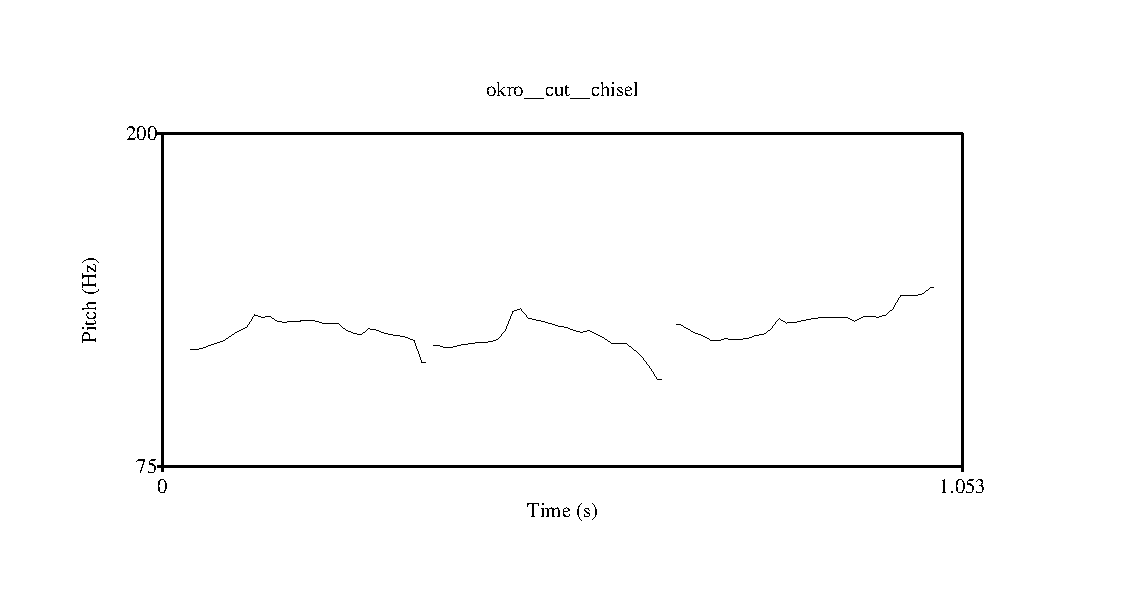
\includegraphics[width=11cm]{Graphic/Pictures/3sounds.pdf}
% %  \caption[Pitch contour of three words]{TAKE NEW! Pitch contour of the words 
% for
% %  `okro', `to cut' and `chisel' (from left to right).  For each word, the 
% contour
% % line starts at the beginning of the first consonant [ŋm] and  stops at the end
% % of the last vowel [a]. \label{fig:PHO-min-triplet}}
% %  \end{figure} 

Distinct tonal melodies at the lexical level provide evidence that a pitch 
distinction affects the meaning of words comprising identical sequences of 
segments.  An example of three different tonal 
melodies, using the minimal triplet, is   {\it ŋmɛ́ná} `okro', {\it ŋmɛ́nà} 
`to cut' and {\it ŋmɛ̀ná}   `chisel'. The same can be said about tonal 
melodies at the phrasal level. Thus, 
the sentences {\it ǹ̩ǹ̩ dí kʊ́ʊ́ rá} `I am eating t.z. ({\it tuo zaafi}, 
type of staple food)' and {\it ǹ̩ dí kʊ̄ʊ̄ rā} `I ate t.z.' are composed of 
the same sequence of segments (except the length of the pronoun in subject 
function), but it is mainly  the tonal melody which distinguishes the former 
utterance from the latter.   Minimal examples involving specific tonal melodies 
are shown  in Section \ref{sec:GRM-trans-intran}.

Based on the evidence of nominal paradigms,  two tones are suggested, i.e. high 
(H) and
low (L).
They are transcribed on segments with an acute and a grave  accent respectively.
Since tones are assigned to moras, light syllables may get a single tone (i.e. H
or L). The heavy syllables may get high (H) or low (L), or either one of the
contour tones, i.e. falling (HL) or rising (LH). A mid tone is often perceived
but no contrast is found  at the lexical level. Provisionally,  the
{mid tone} is said to be a derived tone, that is, a raised low tone  or a 
lowered
high tone. Recall from Section \ref{sec:syllable-types} that the tone-bearing 
units are the vowels, the nasals, the lateral,  and the trill.  


\begin{table}[htp]
\footnotesize

\centering
 \caption{Tonal patterns of singular nouns \label{tab:tone-sing-noun}}


\subfloat[][One light syllable CVC: non-moraic coda]{
\begin{Qtabular}{llp{3.5cm}}
H& hóg	&	bone		\\
H& vʊ́g	&	small god\\	
L& bɔ̀g	&	type of tree	\\	
L& sùk	&	type of tree\\	
\end{Qtabular}
}
\qquad
\subfloat[][One heavy syllable CVC: moraic coda]{
\begin{Qtabular}{llp{3cm}}
H& 		kórː		&seat\\	
L &		sʊ̀lː		&dawadawa\\		
HL&		fʊ́l̀	&	type of creeper \\
LH& 	pòĺ		 & pond	 	\\
\end{Qtabular}
}
\qquad
 \subfloat[][One heavy syllable CVVC]{
\begin{Qtabular}{llp{3cm}}
H & fíél	&	type of grass\\
L & tʃʊ̀àr		& line	\\
HL & báàl	&	male	\\
LH & vàáŋ		& front leg	\\
\end{Qtabular}
}
\qquad
\subfloat[][One heavy syllable CVV]{
\begin{Qtabular}{llp{3cm}}
H&	bíí		& seed  \\
L&	 zùù	&	type of weather	\\	
HL&	lɔ́ʊ̀	& 	hartebeest	\\
LH&	 bìé	&  	child		\\
\end{Qtabular}
}
\qquad
\subfloat[][Two light syllables CVCV]{
\begin{Qtabular}{llp{3cm}}
  
H& bɪ́ná	& 	excrement	\\
L  & bɔ̀là		&elephant	\\
HL&	góŋò	 & 	type of tree	\\
LH & bɪ̀ná & 		year\\	
\end{Qtabular}
}
\qquad
\subfloat[][One heavy CVC: non-moraic coda, one light]{
\begin{Qtabular}{llp{3cm}}

H& tʃéllé		& outlaw	\\		
L & kpã̀nnà	&	lead\\
HL& dántà	&	clan title\\		
LH& kùksó	&	ribs	\\		
\end{Qtabular}
}
\qquad
\subfloat[][One light CV, one heavy CVC]{
\begin{Qtabular}{llp{3cm}}
H & búzóŋ	&	bachelor	\\
HL&  bʊ́zál̀ː	&	type of bird\\
LH & kàtʃíg	&	type of  bird\\
\end{Qtabular}
}
\qquad
\subfloat[][One heavy CVV, one light CV]{
\begin{Qtabular}{llp{3cm}}
 HHH & díésé & 		dream\\
HHL &  kpáásà	&	whip	\\
LHL & kùórù	&	chief	\\
LHH &	tùósó	&	added amount	\\
LLH &	fùòló	&	whistle	\\
LLL &	bʊ̀ɔ̀gà	&	moon	\\
\end{Qtabular}
}
\qquad
\subfloat[][Three light syllables CVCVCV]{
\begin{Qtabular}{llp{3cm}}

HHH &  kásɪ́má	&	corpse uniform	\\ 
HHL &  bélégè	& bathing area	\\
 LHL &  dùlúgù  &	type of bird \\
LLH &  gɛ̀rɛ̀gá	&	sickness\\
 LLL &  dɪ̀gɪ̀nà	&	ear	\\
 LLH &  tʃɪ̀rɪ̀bɔ́		&gun firing pin	\\
LHH &  ʔàmʊ́nʊ́	& 	type of wild cat\\ 
HLL &  kápùtì &  pillow \\

\end{Qtabular}
}
\end{table}

Table \ref{tab:tone-sing-noun} displays  the tonal melodies of the singular noun 
category.  These are words uttered in isolation, so the tones are cut off from 
contextual influences. The subtables are divided according to the moraic content 
of the syllable. The  logical possibilities are accomodated with an example.

These assumption that Chakali has two underlying tones is not controversial: 
\is{Vagla}Vagla, \is{Dɛg}Dɛg, 
\is{Tampulma}Tampulma, 
\is{Sisaala}Sisaala,  and
\is{Pasaale}Pasaale are all described with two tones (\citealt{Rowl65, Crou66, 
Gray69,  Toup95, Crou03})  One finds in this literature high and low tones and a 
considerable number of tone rules. Among them,  a downstep rule, also found in 
Chakali,   lowers a high tone (i.e. {\T ꜜ}H)  when a low tone intervenes between 
 two high tones, e.g. {\it dʊ̃́ʊ̃̀} ({\it sg.} HL), {\it dʊ̃́{\T ꜜ}sá} ({\it 
pl.} HLH). Rule \ref{PHO-downstep} captures the phenomenon. 


\begin{Rule}\label{PHO-downstep}{Downstep}\\
A high tone preceded by a low tone is perceived as lower than a preceding high
tone.\\
 H $\rightarrow$  {\T ꜜ}H  / H  L \_
\end{Rule}



Downdrift is an intonation phenomenon: it is a phrasal property by which a 
sequence of tones is cumulatively lowered; underlyingly though, the tones are 
either high or low. This gradual pitch fall may result in a low tone at the 
beginning of a phrase being as high as a high tone at the end of the phrase. 
Example (\ref{ex:PHO-downdrift}) illustrates the phenomenon. While the first 
line shows how the tones are perceived, the second line provides the lexical  
tones normally associated with each of the words.\footnote{The lack of tone 
rules in the  description is an important level of analysis lacking between 
phrasal intonation and lexical tones,  so example 
(\ref{ex:PHO-downdrift}) must 
be interpreted with vigilance.}


\begin{exe}
\ex\label{ex:PHO-downdrift}

\glll {\T  } {\T  } {\T  } { \T  } {\T }\\
váà tʃʊ̀á dɪ̀á nʊ̀ã́ nɪ́ \\
dog lie house mouth {\postp} \\
\glt  `A dog lies at the entrance of a house.'
\end{exe}



\begin{Rule}\label{PHO-polar-drop}{Polar question drop}\\
A tone (or a series of tones) changes into an extra-low tone at an
utterance-final boundary (condition:  polar question).\\
H*|L*  $\rightarrow$  XL  /  \_ \#\#
\end{Rule}




Generally seen as a discourse function, Chakali has an extra-low tone  which
appears at the end of  polar question (see Section
\ref{sec:GRM-interr-polar}). It is marked with
the diacritic [v̏]. 
Rule \ref{PHO-polar-drop} describes the intonation (drop of pitch) of  polar
questions.



\subsection{Vowel Harmony}
\label{sec:vowel-harmony}

Vowel harmony is a process in  which all the vowels in a particular domain come
to share one or more phonological feature(s).   This agreement  is
triggered in specific phonological domains and  has a
particular direction which is often treated as the spreading of one or more
vowel feature(s).  In Section \ref{sec:vowels},  evidence was provided for the 
establishment of
nine
underlying vowels with five {\sc --atr} and four  {\sc +atr} vowels. This
type of  vowel inventory has been referred to as  a five-height (5Ht) system 
\citep[308]{Casa03},  in which the
feature {\sc atr} is contrastive within both the {\sc +hi} and {\sc [--hi,
--lo]} vowels (see Table \ref{tab:featspec}).  \citet[81--82]{Daku97} and
\citet[312]{Casa03} maintain that it is the most common inventory among
Gur and Kwa languages. 


In Section \ref{sec:LOW-phon-vowel},  the
{\sc --atr} specification of the low vowel at the phonemic level was assumed
  on the basis of its behavior with the set of {\sc --atr} vowels. In
fact, the  realization of the low vowel in vowel harmony suggests that the set
of vowels specified as {\sc --atr}  contains the low vowel. To illustrate
the properties of vowel harmony, let us consider
how they function in  monosyllabic noun roots. Consider the data in
Table
\ref{tab:examples-harmony}.



\begin{table}[!htb]
\small
\centering
\caption{Vowel harmony in noun words\label{tab:examples-harmony}}
 \begin{tabular}{lllll}
\lsptoprule
Root vowel feature & Root &  Singular & Plural & Gloss\\ \midrule

{\sc [+atr, --hi, --lo, --ro]} &sel& sélː&sélé & animal\\
{\sc [+atr, +hi, --lo, --ro]} &bi &bíí &bíé& seed \\
{\sc [+atr, --lo, --ro]} &kie&  kìé 	&kìété	&half of a bird\\
{\sc [+atr, +hi, --lo, +ro]} &ʔul & ʔúl 	& ʔúló 	 
 & 	navel\\
{\sc [+atr, --hi, --lo, +ro]} &hol& hól & hóló & type of tree   \\
{\sc [+atr, --lo, +ro]} &buo& bùó 	& bùósó  &	funeral item\\
{\sc [--atr, +hi, --ro]} &bɪ& bɪ́ɪ́	&	bɪ́á 		&	stone\\
{\sc [--atr,  --hi, --lo, --ro]} &bɛl & bɛ̀ĺ &bɛ́llá & type of tree \\
{\sc [--atr, +hi, --lo, +ro]} & ɲʊg& ɲʊ́g & ɲʊ́gá & crocodile \\
{\sc [--atr,  --hi, --lo, +ro]} & hɔl& hɔ́l & hɔ́lá & piece of charcoal  \\
{\sc [--atr, --lo, +ro]} & bʊɔ& bʊ̀ɔ́	& bʊ̀ɔ̀sá	  &	hole\\
{\sc [--atr, +lo]} &vaa& váá  & vásá & dog \\
{\sc  [--atr, +lo]} &baal& báàl& báàlá& male \\

  \lspbottomrule
 \end{tabular}

\end{table}  

 Chakali is a language with
noun classes (see Section \ref{sec:GRM-noun-classes}). A class is defined as a
pair of singular and plural suffixes
associated with
a particular root.  Looking first at the plural suffixes in Table
\ref{tab:examples-harmony}, it seems that from the underlying nine vowel
inventory of Chakali, only three can occur in such a position, i.e. {\it -a}, 
{\it 
-e},  and {\it -o}. The distribution is such that  when the suffixes occur 
after a
stem containing any member of the set \{ɪ, ɛ, ɔ, ʊ, a\},  they are realized as
{\it -a}.  The plural suffix vowel {\it -e} is realized when the root features 
are
{\sc [+atr, --ro]}, whereas the plural suffix vowel {\it -o} is realized when 
the
root features are {\sc [+atr, +ro]}.  Notice that the height feature(s) of a
vowel is irrelevant in all cases.  Rules \ref{RULE-nc-rule-1} and
\ref{RULE-nc-rule-2} accomodate the surface forms of Table
\ref{tab:examples-harmony}.\footnote{\citet[19, 32--33]{Okee03} states that {\sc
ro}- and {\sc atr}-harmony are both operative in the progressive, future,
egressive, and ingressive of Fante.}


\begin{Rule}\label{RULE-nc-rule-1}{\rm Noun classes realization (1)}\\
A noun class suffix vowel becomes {\sc +atr} if preceded by a {\sc +atr}
stem vowel, and shares the same value for the
feature {\sc ro}  as the one specified on the preceding stem vowel. \\
-V$_{nc}$  $\rightarrow$ [ $\beta${\sc ro},  {\sc +atr},  {\sc --hi}] 
 / [ 
$\beta${\sc ro},
{\sc +atr}] C* \_

\end{Rule}


\begin{Rule}\label{RULE-nc-rule-2}{\rm Noun classes realization (2)}\\
A noun class suffix vowel becomes {\it -a} if the preceding stem vowel is 
{\it ɪ},
{\it ɛ}, {\it ɔ}, {\it ʊ} or {\it a}.\\
-V$_{nc}$ $\rightarrow$ {\sc +lo}  / {\sc --atr} C* \_ 
\end{Rule}


The same rules may be used to account for the vowel
quality of the focus marker (Section \ref{sec:focus-forms}) and  the verbal
suffixes (Section \ref{sec:nasalization-verb-suffix}). Yet, the rules need to
be rewritten in order to be  applicable to wider domains and elements than
those defined in their definition. Rules \ref{RULE-atr} and \ref{RULE-ro} break
down Rules \ref{RULE-nc-rule-1} and \ref{RULE-nc-rule-2} into components able to
be applied to other relevant domains.



\begin{Rule}\label{RULE-atr}{{\sc atr} harmony}\\
A vowel suffix agrees with the {\sc atr} value of   the preceding stem/word 
vowel (domains: noun classes, verbal suffixes, focus marker).\\
V $\rightarrow$ $[\alpha${\sc atr}$]$  / $[\alpha${\sc atr}$]$ C* \_
\end{Rule}


\begin{Rule}\label{RULE-ro}{{\sc ro} harmony}\\
A vowel suffix  agree with the {\sc ro} value of  the   preceding stem/word
 vowel (domains: noun classes, verbal suffixes, focus marker).\\
V $\rightarrow$ [$\alpha${\sc ro}]  / [$\alpha${\sc ro}] C* \_
\end{Rule}

Up to the present, the data suggest that the low vowel is excluded from 
co-occurring with {\sc +atr}  vowels.  So the prediction seems to be that if a 
word contains a {\sc +atr} vowel,  either the low vowel {/{\it a}/} cannot be 
realized and is thus changed by (one of) the above rules, or  the  low vowel is 
banned  altogether from the underlying form. Caution is necessary however since 
complex stem nouns (Section \ref{sec:GRM-com-stem-noun}) are attested containing 
both  low vowels and {\sc +atr} vowels, e.g. {\it pàzèŋ́} ({\it par-zeŋ}, {\sc 
hoe-big})  `big hoe'. Moreover, some multisyllabic words which cannot be treated 
as morphologically complex  due to their lack of morphological transparency do 
appear with both  a {\sc +atr} vowel and  the low vowel, e.g. {\it dáárɪ́}  
`dig' vs.  {\it dààrì}  `be half asleep'. The general tendency is for a low 
vowel to preceed any {\sc +atr} vowels in a word. Taking everything into 
consideration, the phonological and/or morphological domains where one could 
draw the line are still undetermined.



